\chapter{Calculus}
\thispagestyle{fancy}

\keyword{Calculus} is a branch of mathematics that deals with the study of change and motion. It encompasses two main components: differentiation and integration.

\begin{itemize}
	\item \keyword{Differentiation}: This involves finding the rate at which a quantity changes with respect to another variable. The derivative is a fundamental concept in calculus, representing the instantaneous rate of change of a function at a particular point. It helps analyze the behavior of functions, such as finding slopes of curves, determining maximum and minimum points, and understanding the concept of velocity and acceleration.
	
	\item \keyword{Integration}: Integration is the reverse process of differentiation. It involves calculating the accumulation or total amount of a changing quantity over an interval. The integral of a function represents the area under the curve of the function over a given range. It is used to solve problems involving areas, volumes, and quantities related to accumulation, such as calculating total distance traveled from a velocity function or finding the area of a region bounded by a curve.
\end{itemize}

Calculus has numerous real-world applications, ranging from physics and engineering to economics and biology. It provides essential tools for understanding how things change, predicting behavior, and solving complex problems that involve continuous change and motion. Developed independently by Isaac Newton and Gottfried Wilhelm Leibniz in the 17th century, calculus remains a fundamental and powerful branch of mathematics used in various scientific and practical domains.









\section{Definitions and General Differential Equations}
 The derivative of a function represents an infinitesimal change in the function with respect to one of its variables \cite{bib:Wolfram}. 
\begin{defn}[Derivative]{defn:derivative} 
	Let $f:\mathbb{R}\rightarrow\mathbb{R}$. Then the derivative of $f$ with respect to a variable $x$ is given by
	\begin{align*}
	\frac{d}{dx}f(x)\equiv f'(x) \equiv\lim\limits_{\Delta x \rightarrow 0}\frac{f(x+\Delta x)-f(x)}{\Delta x} \equiv \lim\limits_{\Delta x \rightarrow 0}\frac{f(x+\Delta x)-f(x-\Delta x)}{2\Delta x}
	\end{align*}
\end{defn}
Similarly, partial derivatives are defined as derivatives of a function of multiple variables when all but the variable of interest are held fixed during the differentiation \cite{bib:Wolfram}. 
\begin{defn}[Partial Derivative]{defn:partial derivative}
	Let $f:\mathbb{R}^z\rightarrow\mathbb{R}$, with $z \in \mathbb{N}$. Then the partial derivative of $f$ with respect to a variable $x_m$ is given by
	\begin{align*}
	\frac{\partial}{\partial x_m}f(x_1,\dots,x_n) \equiv \lim\limits_{\Delta x \rightarrow 0}\frac{f(x_1,\dots,x_m+\Delta x, \dots,x_n)-f(x_1,\dots,x_m,\dots,x_n)}{\Delta x}
	\end{align*}
\end{defn}
A few rules from definition \ref{defn:derivative} can be defined.
\begin{theo}[Distributive Property Of Derivatives]{thm:derivative_distributive}
	Let $g:\mathbb{R}\rightarrow\mathbb{R}$, and $h:\mathbb{R}\rightarrow\mathbb{R}$ be continuous functions with $f(x)=g(x)+h(x)$. Then the derivative of $f$ with respect to the variable $x$ is 
	\begin{align*}
	\frac{d}{dx}f(x)=\frac{d}{dx}\big(g(x)+h(x)\big) = \frac{d}{dx}g(x)+\frac{d}{dx}g(x).
	\end{align*} 
\end{theo}

\begin{proof}[Proof for theorem \ref{thm:derivative_distributive}]
	Let $g:\mathbb{R}\rightarrow\mathbb{R}$, and $h:\mathbb{R}\rightarrow\mathbb{R}$ be continuous functions with $f(x)=g(x)+h(x)$. Then, by the definition of a derivative, we have
	\begin{align*}
	\frac{d}{dx}f(x)&=\lim\limits_{\Delta x \rightarrow 0}\frac{f(x+\Delta x)-f(x)}{\Delta x} \\
	&=\lim\limits_{\Delta x \rightarrow 0}\frac{(g+h)(x+\Delta x)-(g+h)(x)}{\Delta x} \\
	&=\lim\limits_{\Delta x \rightarrow 0}\frac{g(x+\Delta x)+h(x+\Delta x)-g(x)-h(x)}{\Delta x} \\
	&=\lim\limits_{\Delta x \rightarrow 0}\bigg(\frac{g(x+\Delta x)-g(x)}{\Delta x}+\frac{h(x+\Delta x)-h(x)}{\Delta x}\bigg) \\
	&=\lim\limits_{\Delta x \rightarrow 0}\frac{g(x+\Delta x)-g(x)}{\Delta x}+\lim\limits_{\Delta x \rightarrow 0}\frac{h(x+\Delta x)-h(x)}{\Delta x} \\
	&= \frac{d}{dx}g(x)+\frac{d}{dx}h(x).
	\end{align*}
	Thus, by simple manipulation we've shown
	\begin{align*}
	\frac{d}{dx}f(x)= \frac{d}{dx}g(x)+\frac{d}{dx}g(x).
	\end{align*}
\end{proof}
If we want to take the derivative of a function
Given a general polynomial function, we can give the following differentiation rule.
\begin{theo}[Polynomial Derivatives]{deriving_ordinary_polynomial}
	Let $f:\mathbb{R}\rightarrow\mathbb{R}$ be a function with $f(x)=c_nx^n+c_{n-1}x^{n-1}+\cdots++C_2x^2+c_1x+c_0$, where $c_n$ is constant for all $n$. Then
	\begin{align*}
	\frac{d}{dx}f(x)=f'(x)=nc_nx^{n-1}+(n-1)c_{n-1}x^{n-2}+\cdots+2c_2x+c_1
	\end{align*}
\end{theo}
\begin{proof}[Proof for theorem \ref{deriving_ordinary_polynomial}]
	Let $f:\mathbb{R}\rightarrow\mathbb{R}$ be a function with $f(x)=c_nx^n+c_{n-1}x^{n-1}+\cdots++C_2x^2+c_1x+c_0$, where $c_n$ is constant for all $n$. Let $g_n(x)=c_nx^n$. By theorem 1.1, we know that $f'(x)=g'_n(x)+g'_{n-1}(x)+\cdots+g_1(x)+g_0(x)$. Therefore, if we can prove $p(x)=Cx^n\implies p'(x)=nCx^n$, then this directly implies each term of $f(x)$ will have a derivative of equivalent form.
	Starting with $p$, we must first note that $p(x)=Cx^n$ and $p(x+h)=C(x+h)^n$. Inserting these into the limit definition will give us 
	\begin{align*}
	p'(x) = \lim_{h\to0} \frac{p(x+h)-p(x)}{h} = \lim_{h\to0} \frac{C(x+h)^n-Cx^n}{h}.
	\end{align*}
	As we can see, we can expand $(x+h)^n$ using the binomial theorem. This gives us
	\begin{align*}
	C\lim_{h\to0} \frac{\sum\limits_{k=0}^{n}{{n}\choose{k}}x^{n-k}h^k-x^n}{h}.
	\end{align*}
	If we denote $a_k={{n}\choose{k}}=\frac{n!}{k!(n-k)!}$, then expand the summation, we get
	\begin{align}
	C\lim_{h\to0}\frac{\sum\limits_{k=0}^{n}a_kx^{n-k}h^k-x^n}{h}=C\lim_{h\to0}\frac{a_0x^{n}+a_1x^{n-1}h+a_2x^{n-2}h^2+a_3x^{n-3}h^3+\dots+a_kx^{n-k}h^k-x^n}{h}.
	\end{align}
	If we determine $a_0$ and $a_1$ we get
	\begin{align}
	a_0 &=\frac{n!}{0!n!}=1 \\
	a_1 &=\frac{n!}{1!(n-1)!} =\frac{n!(n)}{(n-1)!(n)}=\frac{n!(n)}{n!}=n.
	\end{align}
	Inserting equations (1.2) and (1.3) into (1.1) yields
	\begin{align*}
	C\lim_{h\to0}\frac{x^n+nx^{n-1}h+a_2x^{n-2}h^2+a_3x^{n-3}h^3+\dots+a_kx^{n-k}h^k-x^n}{h}.
	\end{align*}
	Then, we see that the first and last terms add to zero
	\begin{align*}
	C\lim_{h\to0}\frac{nx^{n-1}h+a_2x^{n-2}h^2+a_3x^{n-3}h^3+\dots+a_kx^{n-k}h^k}{h}.
	\end{align*}
	From here, we simplify by dividing by $h$ and take the limit as $h \to 0$
	\begin{align*}
	C\lim_{h\to0}nx^{n-1}+a_2x^{n-2}h+a_3x^{n-3}h^2+\dots+a_kx^{n-k}h^{k-1}=Cnx^{n-1}.
	\end{align*}
	Hence, we have determined that $p'(x)=Cnx^{n-1}$ which directly implies
	\begin{align*}
	\frac{d}{dx}f(x)=f'(x)=nc_nx^{n-1}+(n-1)c_{n-1}x^{n-2}+\cdots+2c_2x+c_1
	\end{align*}
\end{proof}

Consider the basic product rule of a differential equation. The product rule is given by
\begin{theo}[Product Rule]{thm:product rule}
	Let $f:\mathbb{R}\rightarrow\mathbb{R}$ such that $f(x)$ and $g(x)$ are continuous functions of the variable $x$. We can then say
	\begin{align*}
		\frac{d}{dx}f(x)g(x)=g(x)\frac{d}{dx}f(x)+f(x)\frac{d}{dx}g(x)=f'(x)g(x)+f(x)g'(x)
	\end{align*}
\end{theo}
\begin{proof}[Proof for theorem \ref{thm:product rule}]
	Let $f:\mathbb{R}\rightarrow\mathbb{R}$ such that $f(x)$ and $g(x)$ are continuous functions of the variable $x$. By the definition of the derivative, we have
	\begin{align*}
		\frac{d}{dx}f(x)g(x)&=\lim\limits_{\Delta x \rightarrow 0}\frac{f(x+\Delta x)g(x+\Delta x)-f(x)g(x)}{\Delta x} \\
		&=\lim\limits_{\Delta x \rightarrow 0}\frac{f(x+\Delta x)g(x+\Delta x)-f(x+\Delta x)g(x)+f(x+\Delta x)g(x)-f(x)g(x)}{\Delta x} \\
		&=\lim\limits_{\Delta x \rightarrow 0}\frac{f(x+\Delta x)\big(g(x+\Delta x)-g(x)\big)+g(x)\big(f(x+\Delta x)-f(x)\big)}{\Delta x} \\
		&=\lim\limits_{\Delta x \rightarrow 0}f(x+\Delta x)\frac{g(x+\Delta x)-g(x)}{\Delta x}+\lim\limits_{\Delta x \rightarrow 0}g(x)\frac{f(x+\Delta x)-f(x)}{\Delta x} \\
		&=f(x)\frac{d}{dx}g(x)+g(x)\frac{d}{dx}f(x) \\&=f'(x)g(x)+f(x)g'(x).
	\end{align*}
\end{proof}
It is thus clear that given two continuous functions of $x$, say $f(x)$ and $g(x)$, the derivative follows as
\begin{align}
	\frac{d}{dx}f(x)g(x) &= g(x)\frac{d}{dx}f(x)+f(x)\frac{d}{dx}g(x) \\
 		             &= f(x)g'(x)+g(x)f'(x). \label{product_rule_n1}
\end{align}
Following this, the second derivative is given by
\begin{align}
	\frac{d^2}{dx^2}f(x)g(x)&=\frac{d}{dx}\bigg(g(x)\frac{d}{dx}f(x)\bigg)+\frac{d}{dx}\bigg(f(x)\frac{d}{dx}g(x)\bigg) \\
	&=\frac{d}{dx}f(x)\frac{d}{dx}g(x)+g(x)\frac{d^2}{dx^2}f(x)+f(x)\frac{d^2}{dx^2}g(x)+\frac{d}{dx}f(x)\frac{d}{dx}g(x) \\
	&=2\frac{d}{dx}f(x)\frac{d}{dx}g(x)+g(x)\frac{d^2}{dx^2}f(x)+f(x)\frac{d^2}{dx^2}g(x) \\
	&= f(x)g''(x)+2f'(x)g'(x)+f''(x)g(x). \label{product_rule_n2}
\end{align}
Similarly, the third derivative is given by
\begin{align}
	\frac{d^3}{dx^3}f(x)g(x)&=\frac{d}{dx}\bigg(2\frac{d}{dx}f(x)\frac{d}{dx}g(x)+g(x)\frac{d^2}{dx^2}f(x)+f(x)\frac{d^2}{dx^2}g(x)\bigg) \\
	&=\frac{d}{dx}\bigg(2\frac{d}{dx}f(x)\frac{d}{dx}g(x)\bigg)+\frac{d}{dx}\bigg(g(x)\frac{d^2}{dx^2}f(x)\bigg)+\frac{d}{dx}\bigg(f(x)\frac{d^2}{dx^2}g(x)\bigg).
\end{align}
This derivative can be done in parts to help keep track of what is being done. Let us denote each term in the above sum as $h_1(x)$, $h_2(x)$ and $h_3(x)$ respectively. Then we have
\begin{align}
	h_1(x)&= \frac{d}{dx}\bigg(2\frac{d}{dx}f(x)\frac{d}{dx}g(x)\bigg) \\
	h_2(x)&=\frac{d}{dx}\bigg(g(x)\frac{d^2}{dx^2}f(x)\bigg) \\
	h_3(x)&=\frac{d}{dx}\bigg(f(x)\frac{d^2}{dx^2}g(x)\bigg).
\end{align}
Simplifying these expressions then gives
\begin{align}
	h_1(x)&= \bigg(2\frac{d^2}{dx^2}f(x)\frac{d}{dx}g(x)+2\frac{d}{dx}f(x)\frac{d^2}{dx^2}g(x)\bigg) \\
	h_2(x)&=\bigg(\frac{d}{dx}g(x)\frac{d^2}{dx^2}f(x)+g(x)\frac{d^3}{dx^3}f(x)\bigg) \\
	h_3(x)&=\bigg(\frac{d}{dx}f(x)\frac{d^2}{dx^2}g(x)+f(x)\frac{d^3}{dx^3}g(x)\bigg).
\end{align}
Then, adding these three expressions together gives us
\begin{align}
	\frac{d^3}{dx^3}f(x)g(x)&=f(x)\frac{d^3}{dx^3}g(x)+3\frac{d}{dx}f(x)\frac{d^2}{dx^2}g(x)+3\frac{d^2}{dx^2}f(x)\frac{d}{dx}g(x)+g(x)\frac{d^3}{dx^3}f(x)\\
	&=f(x)g'''(x)+3f'(x)g''(x)+3f''(x)g'(x)+f'''(x)g(x). \label{product_rule_n3}
\end{align}
Using the product rule, a nice pattern seems to be emerging as we continually apply it to the same function. From equations (\ref{product_rule_n1}), (\ref{product_rule_n2}) and (\ref{product_rule_n3}), we can see that it appears to be a similar pattern as when applying the binomial expansion theorem. As a reminder, the binomial expansion theorem is
\begin{align}
	(a+b)^n&=\sum_{k=0}^{n}{{n}\choose{k}}a^{n-k}b^k \\
	{{n}\choose{k}}&= \frac{n!}{k!(n-k)!}.
\end{align}
If we observe the first three terms of this (with $n=1,2,3$), we have
\begin{align}
	(a+b)^1&=a+b\\
	(a+b)^2&= a^2+2ab+b^2 \\
	(a+b)^3 &= a^3+3a^2b+3ab^2+b^3.
\end{align}
Comparing this to the three equations in questions allows us to notice interesting similarities. If we expand this to $n$ we have
\begin{align}
	(a+b)^n=a^nb^0+{{n}\choose{1}}a^{n-1}y^1+\cdots+{{n}\choose{n-1}}ab^{k-1}+a^0b^k. \label{binomial_expansion_00}
\end{align}
Now, let $a=\frac{d}{dx}g(x)$ and $b=\frac{d}{dx}f(x)$. If we temporarily define\footnote{This is solely for an easy way of noticing the similarities in the formulas, these equations do not necessarily hold and are not used once the equations are expanded.} the following conditions
\begin{align}
	\bigg(\frac{d}{dx}h(x)\bigg)^n&:=\frac{d^n}{dx^n}h(x) \label{redefinition_derivative_00}\\
	\frac{d}{dx}g(x)+\frac{d}{dx}f(x) &:= \frac{d}{dx}g(x)f(x) \label{redefinition_derivative_01},
\end{align}
then inserting $a$ and $b$ into equation (\ref{binomial_expansion_00}) gives
\begin{align}
	\bigg[\frac{d}{dx}g(x)+\frac{d}{dx}f(x) \bigg]^n=\bigg(\frac{d}{dx}g(x)\bigg)^n\bigg(\frac{d}{dx}f(x)\bigg)^0+{{n}\choose{1}}\bigg(\frac{d}{dx}g(x)\bigg)^{n-1}\bigg(\frac{d}{dx}f(x)\bigg)^1+\cdots \\ \cdots+{{n}\choose{n-1}}\bigg(\frac{d}{dx}g(x)\bigg)\bigg(\frac{d}{dx}f(x)\bigg)^{n-1}+\bigg(\frac{d}{dx}g(x)\bigg)^0\bigg(\frac{d}{dx}f(x)\bigg)^n.
\end{align}
Simplifying the above expression gives us
\begin{align}
	\frac{d^n}{dx^n}g(x)f(x)=f(x)\frac{d^n}{dx^n}g(x)+{{n}\choose{1}}\frac{d^{n-1}}{dx^{n-1}}g(x)\frac{d}{dx}f(x)+\cdots \\
	\cdots+{{n}\choose{n-1}}\frac{d}{dx}g(x)\frac{d^{n-1}}{dx^{n-1}}f(x)+g(x)\frac{d^n}{dx^n}f(x).
\end{align}
Therefore, we can see that with our re-definitions in equations (\ref{redefinition_derivative_00}) and (\ref{redefinition_derivative_01}), it appears that the $n^{\textrm{th}}$ derivative of something using the product rule can be expressed using the binomial expansion theorem. At least to $n=3$ we can see from above that this is accurate. If we want to determine if this works for all values of $n$, we can try a proof by induction. Before going any further, since this may be a large amount of work for such a simple idea, let us quickly have a sanity check. We claim that the terms of the product rule can be expanded using the binomial theorem. It is important to note that when taking the product rule of an expression, you get two new expressions. Then, taking the product rule again will double those two into four, and then those four into eight, and so on. So we can see that each product rule doubles the number of terms we have. The binomial coefficient is used when we have like terms to combine them. If we were to add up each binomial coefficient in the sum, we should then see that each sum of coefficients is the same number of terms we would get as if we doubled our expression each time. If this were not so then our situation would have a flaw. In other words, it must hold true that
\begin{align}
	\sum_{i=0}^{n}{{n}\choose{k}} = 2^n.
\end{align}
This indeed is true. See theorem \ref{thm:Summing Over All binomial coefficients}. Now, we know from equations (\ref{product_rule_n1}), (\ref{product_rule_n2}) and (\ref{product_rule_n3}) that cases $n=1,2,3$ all hold. Next, if we assume that for any $n=k$ that
\begin{align}
	\frac{d^k}{dx^k}g(x)f(x)&=f(x)\frac{d^k}{dx^k}g(x)+{{k}\choose{1}}\frac{d^{k-1}}{dx^{k-1}}g(x)\frac{d}{dx}f(x)+\cdots \nonumber\\
	&\hspace{1cm}\cdots+{{k}\choose{k-1}}\frac{d}{dx}g(x)\frac{d^{k-1}}{dx^{k-1}}f(x)+g(x)\frac{d^k}{dx^k}f(x) \\
	&=\sum_{i=0}^{k}{{k}\choose{i}}\bigg[\frac{d^i}{dx^i}f(x) \bigg]\bigg[\frac{d^{k-i}}{dx^{k-i}}g(x) \bigg] \label{repeating_product_rule_final_k}
\end{align}
holds true, we can then determine if it holds true for $n=k+1$. This gives
\begin{align}
	\frac{d^{k+1}}{dx^{k+1}}g(x)f(x)&=f(x)\frac{d^{k+1}}{dx^{k+1}}g(x)+{{{k+1}}\choose{1}}\frac{d^{k}}{dx^{k}}g(x)\frac{d}{dx}f(x)+\cdots \nonumber\\
	&\hspace{1cm}\cdots+{{k+1}\choose{k}}\frac{d}{dx}g(x)\frac{d^{k}}{dx^{k}}f(x)+g(x)\frac{d^{k+1}}{dx^{k+1}}f(x) \\
	&=\sum_{i=0}^{k+1}{{k+1}\choose{i}}\bigg[\frac{d^i}{dx^i}f(x) \bigg]\bigg[\frac{d^{k+1-i}}{dx^{k+1-i}}g(x) \bigg].
\end{align}
If we were to manually evaluate the $n=k+1$ term of this expression we would have
\begin{align}
	\frac{d}{dx}\frac{d^{k}}{dx^{k}}g(x)f(x)= \frac{d}{dx}\sum_{i=0}^{k}{{k}\choose{i}}\bigg[\frac{d^i}{dx^i}f(x) \bigg]\bigg[\frac{d^{k-i}}{dx^{k-i}}g(x) \bigg].
\end{align}
Since differentiating is distributive (by theorem \ref{thm:derivative_distributive}), we can evaluate each term of this sum and compare it to (32) and (33). Doing this, we can use the product rule to first get
\begin{align}
	\frac{d^{k+1}}{dx^{k+1}}g(x)f(x)=\sum_{i=0}^{k}{{k}\choose{i}}\bigg[\frac{d^{i+1}}{dx^{i+1}}f(x) \bigg]\bigg[\frac{d^{k-i}}{dx^{k-i}}g(x) \bigg]+{{k}\choose{i}}\bigg[\frac{d^i}{dx^i}f(x) \bigg]\bigg[\frac{d^{k+1-i}}{dx^{k+1-i}}g(x) \bigg]. 
\end{align}
From here, writing out the series explicitly allows us to combine terms in a useful matter. This would obviously be tedious to write out so let us denote each term by $a_i$, for any $i^{\textrm{th}}$ term in the summation. Writing out a few of the terms then gives
\begin{align}
	a_0&={{k}\choose{0}}\bigg[\frac{d^{1}}{dx^{1}}f(x) \bigg]\bigg[\frac{d^{k}}{dx^{k}}g(x) \bigg]+{{k}\choose{0}}f(x)\bigg[\frac{d^{k+1}}{dx^{k+1}}g(x) \bigg] \\
	a_1&={{k}\choose{1}}\bigg[\frac{d^{2}}{dx^{2}}f(x) \bigg]\bigg[\frac{d^{k-1}}{dx^{k-1}}g(x) \bigg]+{{k}\choose{1}}\bigg[\frac{d}{dx}f(x) \bigg]\bigg[\frac{d^{k}}{dx^{k}}g(x) \bigg] \\
	a_2&={{k}\choose{2}}\bigg[\frac{d^{3}}{dx^{3}}f(x) \bigg]\bigg[\frac{d^{k-2}}{dx^{k-2}}g(x) \bigg]+{{k}\choose{2}}\bigg[\frac{d^2}{dx^2}f(x) \bigg]\bigg[\frac{d^{k-1}}{dx^{k-1}}g(x) \bigg]\\
	&\vdots \nonumber\\
	a_{k-2}&={{k}\choose{k-2}}\bigg[\frac{d^{k-1}}{dx^{k-1}}f(x) \bigg]\bigg[\frac{d^{2}}{dx^{2}}g(x) \bigg]+{{k}\choose{k-2}}\bigg[\frac{d^{k-2}}{dx^{k-2}}f(x) \bigg]\bigg[\frac{d^{3}}{dx^{3}}g(x) \bigg]\\
	a_{k-1}&={{k}\choose{k-1}}\bigg[\frac{d^{k}}{dx^{k}}f(x) \bigg]\bigg[\frac{d}{dx}g(x) \bigg]+{{k}\choose{v}}\bigg[\frac{d^{k-1}}{dx^{k-1}}f(x) \bigg]\bigg[\frac{d^{2}}{dx^{2}}g(x) \bigg]\\
	a_k&={{k}\choose{k}}\bigg[\frac{d^{k+1}}{dx^{k+1}}f(x) \bigg]g(x)+{{k}\choose{k}}\bigg[\frac{d^k}{dx^k}f(x) \bigg]\bigg[\frac{d}{dx}g(x) \bigg].
\end{align}
At this point, it becomes obvious as to why the $f^{(n)}(x)$ notation of a derivative was invented, and switching over will greatly help in our next step. Changing our notation gives us 
\begin{align}
	a_0&={{k}\choose{0}}f^{(1)}(x) g^{(k)}(x)+{{k}\choose{0}}f(x)g^{(k+1)}(x) \label{repeating_product_rule_a0}\\
	a_1&={{k}\choose{1}}f^{(2)}(x) g^{(k-1)}(x) +{{k}\choose{1}}f^{(1)}(x) g^{(k)}(x) \\
	a_2&={{k}\choose{2}}f^{(3)}(x) g^{(k-2)}(x) +{{k}\choose{2}}f^{(2)}(x) g^{(k-1)}(x) \\
	&\vdots \nonumber\\
	a_{k-2}&={{k}\choose{k-2}}f^{(k-1)}(x) g^{(2)}(x) +{{k}\choose{k-2}}f^{(k-2)}(x) g^{(3)}(x)\\
	a_{k-1}&={{k}\choose{k-1}}f^{(k)}(x) g^{(1)}(x)+{{k}\choose{k-1}}f^{(k-1)}(x) g^{(2)}(x)\\
	a_k&={{k}\choose{k}}f^{(k+1)}(x) g(x)+{{k}\choose{k}}f^{(k)}(x)g^{(1)}(x). \label{repeating_product_rule_ak}
\end{align}
Our end goal is to get this expression to be in the same form as in equation (\ref{repeating_product_rule_final_k}). If we first re-write equation (\ref{repeating_product_rule_final_k}) using $f^{(n)}(x)$ notation, we can easily see what our end goal is. This is
\begin{align}
	\sum_{i=0}^{k+1}{{k+1}\choose{i}}f^{(i)}(x) g^{(k+1-i)}(x) \label{repeating_product_rule_final}.
\end{align}
The next step is then summing expressions (\ref{repeating_product_rule_a0}) through (\ref{repeating_product_rule_ak}), then determining if what we get is equivalent to equation (\ref{repeating_product_rule_final}). Let $\Upsilon=a_0+a_1+\cdots+a_{k-1}+a_k$, then we have
\begin{align}
	\Upsilon&={{k}\choose{0}}f(x)g^{(k+1)}(x)+{{k}\choose{0}}f^{(1)}(x)g^{(k)}(x)+{{k}\choose{1}}f^{(1)}(x)g^{(k)}(x)+\cdots \nonumber\\
	&\hspace{1cm}\cdots+{{k}\choose{k}}f^{(k)}(x)g^{(1)}(x)+{{k}\choose{k-1}}f^{(k)}(x)g^{(1)}(x)+{{k}\choose{k}}f^{(k+1)}(x)g(x) \\
	&={{k}\choose{0}}f(x)g^{(k+1)}(x)+\bigg[{{k}\choose{0}}+{{k}\choose{1}} \bigg]f^{(1)}(x)g^{(k)}(x)+\cdots \nonumber\\
	&\hspace{1cm}\cdots+\bigg[{{k}\choose{k-1}}+{{k}\choose{k}} \bigg]f^{(k)}(x)g^{(1)}(x)+{{k}\choose{k}}f^{(k+1)}(x)g(x)\\
	&=\sum_{i=0}^{k+1}\bigg[{{k}\choose{i-1}}+{{k}\choose{i}} \bigg]f^{(i)}(x)g^{(k+1-i)}(x). \label{repeating_product_rule_00}
\end{align}
Using the definition of the binomial coefficient and the derivation in (7), if we let $k=m-1 \implies m=k+1$, we can re-write the binomial coefficient in equation (\ref{repeating_product_rule_00}) as follows.
\begin{align}
	{{k}\choose{i-1}}+{{k}\choose{i}}={{m-1}\choose{i-1}}+{{m-1}\choose{i}}={{m}\choose{i}}={{k+1}\choose{i}}.
\end{align}
Thus, equation (\ref{repeating_product_rule_00}) becomes
\begin{align}
	\Upsilon=\sum_{i=0}^{k+1}{{k+1}\choose{i}}f^{(i)}(x)g^{(k+1-i)}(x).
\end{align}
Now, $\Upsilon=a_0+a_1+\cdots+a_{k-1}+a_k=(35)$ which we have shown is equivalent to equation (\ref{repeating_product_rule_00}). Therefore, we can conclude that (28) holds for all $n\in\mathbb{N}$, which allows us to tidy our work up as a theorem.
\begin{theo}[Repeating Product Rule]{thm:repeating product rule}
	Let $f:\mathbb{R}\rightarrow\mathbb{R}$ and $g:\mathbb{R}\rightarrow\mathbb{R}$ be continuous and differentiable functions of the variable $x$. Then the $m^{\textrm{th}}$ derivative of $f(x)g(x)$ with respect to $x$ is
	\begin{align*}
		\frac{d^m}{dx^m}f(x)g(x)=\sum_{i=0}^{n}{{n}\choose{i}}\bigg[\frac{d^i}{dx^i}f(x) \bigg]\bigg[\frac{d^{n-i}}{dx^{n-i}}g(x) \bigg].
	\end{align*}
\end{theo}



Consider a division of two functions rather than multiplication. The product rule can be used to derive what is referred to as the \keyword{quotient rule}. Begin by taking two arbitrary functions that are continuous and differentiable $f(x)$ and $g(x)$. What we want to find is $\frac{d}{dx} \frac{f(x)}{g(x)}$. We begin by applying the product rule from theorem \ref{thm:product rule}, which gives
\begin{align}
	\frac{d}{dx} \frac{f(x)}{g(x)} = f(x)\left[\frac{d}{dx} \frac{1}{g(x)}\right] + \frac{1}{g(x)}\left[\frac{d}{dx} f(x)\right] \label{quotient_rule_00}.
\end{align}
Let $u(x)=\frac{1}{g(x)}$. We want to determine $u'(x)$ in order to simplify equation (\ref{quotient_rule_00}). From the definition of $u(x)$, we can then say $u(x)g(x)=1$. The derivative of a constant value is just zero, so if we differentiate both sides (by yet again applying the product rule from theorem \ref{thm:product rule}), we get
\begin{align}
	\frac{d}{dx}u(x)g(x)=\frac{d}{dx}1 \implies u(x)g'(x) + u'(x)g(x)=0.
\end{align}
Solving this for $u'(x)$ gives us $\frac{d}{dx} \frac{1}{g(x)}$ which we is then equal to 
\begin{align}
	u'(x) = \frac{d}{dx} u(x) = \frac{d}{dx} \frac{1}{g(x)} = \frac{-u(x)g'(x)}{g(x)} = -\frac{g'(x)}{g(x)^2} \label{quotient_rule_01}.
\end{align}
By taking equation (\ref{quotient_rule_01}) and substituting it into equation (\ref{quotient_rule_00}), we get
\begin{align}
	\frac{d}{dx} \frac{f(x)}{g(x)} = f(x)\left[-\frac{g'(x)}{g(x)^2}\right] + \frac{1}{g(x)}f'(x) = -\frac{f(x)g'(x)}{g(x)^2}+ \frac{g(x)f'(x)}{g(x)^2} = \frac{f'(x)g(x)-f(x)g'(x)}{g(x)^2}.
\end{align}

\begin{theo}[Quotient Rule]{thm:quotient rule}
	Let $f:\R \to \R$ and $g: \R\to\R$ be continuous and differentiable functions of the variable $x$. Then the derivative of $\frac{f(x)}{g(x)}$ with respect to $x$ is
	\begin{align}
		\frac{d}{dx} \frac{f(x)}{g(x)} = \frac{f'(x)g(x)-f(x)g'(x)}{g(x)^2}.
	\end{align}
\end{theo}
A special case of this quotient rule is when the numerator is $1$. This can be seen in equation (\ref{quotient_rule_00}). For simplicity, I will drop the "$(x)$" and assume functions with a single variable here. Taking consecutive derivatives of this give
\begin{align}
	\frac{d}{dx}\frac{1}{g} &= \frac{-g'}{g^2} \label{d/dx 1/g 1}\\
	\frac{d^2}{dx^2}\frac{1}{g} &= \frac{d}{dx}\frac{-g'}{g^2} = -\frac{d}{dx}g'\frac{1}{g^2} = -\frac{g''}{g^2}-g'\left(\frac{-2gg'}{g^4}\right) = -\frac{g''}{g^2}+\frac{2g'^2}{g^3} \label{d/dx 1/g 2}\\
	\frac{d^3}{dx^3}\frac{1}{g} &= \frac{d}{dx}\left(-\frac{g''}{g^2}+\frac{2g'^2}{g^3}\right) =- \frac{g'''}{g^2} - g''\frac{d}{dx}\frac{1}{g^2} +  \frac{4g'g''}{g^3} + 2g'^2\frac{d}{dx}\frac{1}{g^3}  \nonumber \\&= -\frac{g'''}{g^2}-g''\left(\frac{-2gg'}{g^4}\right)+\frac{4g'g''}{g^3}+2g'^2\left(\frac{-3g^2g'}{g^6}\right) \nonumber\\
	&= -\frac{g'''}{g^2}+\frac{2g'g''}{g^3}+\frac{4g'g''}{g^3}-\frac{6g'^3}{g^4} \nonumber\\
	&=\frac{6g'g''}{g^3}-\frac{6g'^3}{g^4}-\frac{g'''}{g^2} \label{d/dx 1/g 3}\\
	\frac{d^4}{dx^4}\frac{1}{g} &= \frac{d}{dx}\left(\frac{6g'g''}{g^3}-\frac{6g'^3}{g^4}-\frac{g'''}{g^2}\right) \nonumber \\
	&= 6g'g''\frac{d}{dx}\frac{1}{g^3}+\frac{1}{g^3}\frac{d}{dx}6g'g''-6g'^3\frac{d}{dx}\frac{1}{g^4}-\frac{1}{g^4}\frac{d}{dx}6g'^3-g'''\frac{d}{dx}\frac{1}{g^2}-\frac{1}{g^2}\frac{d}{dx}g'''\nonumber \\
	&= \frac{-18g'^2g''}{g^4}+\frac{6g'g'''+6g''^2}{g^3}+\frac{24g'^4}{g^5}-\frac{18g'^2g''}{g^4}+\frac{2g'g'''}{g^3}-\frac{g^{(4)}}{g^2}\nonumber \\
	&= \frac{-36g'^2g''}{g^4}+\frac{8g'g'''}{g^3}+\frac{6g''^2}{g^3}+\frac{24g'^4}{g^5}-\frac{g''''}{g^2} \label{d/dx 1/g 4}\\
	\frac{d^5}{dx^5}\frac{1}{g} &= \frac{-g^{(5)}}{g^2}-\frac{120g'^5}{g^6}+\frac{10g^{(4)}g'}{g^3}+\frac{20g'''g''}{g^3}-\frac{60g'''g'^2}{g^4}+\frac{240g'^3g''}{g^5}-\frac{90g'g''^2}{g^4},\label{d/dx 1/g 5}
\end{align}
and so on. Notice on that last one I spared the algebra. to find a pattern in this sequence, a few things can be noted. First. The factor of $\left(\frac{1}{g}\right)^m$ is common in every term. The maximum $m$ value here appears to be equal to $m=n+1$, where $n$ is the number of derivatives performed. There also seem to be at least one term for each $m$ value except for $m=1$ (for example, in equation (\ref{d/dx 1/g 1}) there is only a $g^2$ term, with a maximum $m=2$, but in equation (\ref{d/dx 1/g 5}), there are $m=2,3,4,5,\text{ and }6$ terms). Next, there is a common occurrence of $\frac{d^k}{dx^k}g$ terms, where the highest $k$ value appears to be $k=n$ in each derivative. There does not seem to be an immediate pattern with the coefficients. For each $\frac{d^n}{dx^n}$, there is also a $-\frac{g^{(n)}}{g^2}$ term.

Using these observations, we can begin to construct a potential formula to represent this pattern. It must be a sum of some kind, since it has summed terms. It must contain one term for each $\left(\frac{1}{g}\right)^m$ for all $1\leq m \leq n+1$. Each term will have some coefficient, which will likely be dependent on $m$, $n$, or both $m$ and $n$. And each term will have some product of $g^{(i)}$ terms. We can thus guess our formula to look something like
\begin{align}
	\frac{d^n}{dx^n}\frac{1}{g} \overset{?}{=} \sum_{m=0}^{n}\frac{C(n,m)}{g^{m+1}}G( g^{(i)}|i \leq n \in \N^+), \label{d/dx 1/g guess 00}
\end{align}
where $C(n,m)$ is some coefficient function dependent on $n$ and $m$, and $G(g^{(i)}|i \leq n \in \N^+) \equiv G(g^{(1)}, g^{(2)},...,g^{(n)})$ is some function which is a product of the repeated derivatives of $g(x)$ in some combination. Some possible steps to determine this formula better would of course be to then determine $G$ and $C$. We know the above equations involve deriving $g(x)$. With a careful and lucky observation, $G$ can be determined. Consider this derivative for a moment $\frac{d}{dx} g(x) =  g'(x)$. If we take consecutive derivatives, we simply get $\frac{d^i}{dx^i} g(x) =  g^{(i)}(x)$. Now consider this derivative for a moment $\frac{d}{dx} g(x)^2 =  2g(x)g'(x)$. When there are multiple terms of our function, the consecutive derivatives require the product rule, which would give $\frac{d^2}{dx^2} g(x)^2 =  2g(x)g''(x)+2g'(x)^2$. Careful observation will reveal that this corresponds to the derivatives in equation (\ref{d/dx 1/g 2}), where as the first derivative of $g(x)$ corresponds to the coefficients in equation (\ref{d/dx 1/g 1}). Taking a third derivative of $g(x)^2$ gives $\frac{d^3}{dx^3} g(x)^2 =  2g(x)g'''(x)+6g'(x)g''(x)$. This only closely correlates to equation (\ref{d/dx 1/g 3}). If instead we take the third derivative of $g(x)^3$, we have $\frac{d^3}{dx^3} g(x)^3 =  3(g(x)^2g'''(x)+2g'(x)^3 +6g'(x)g''(x)$, which indeed correlates to the coefficients in equation (\ref{d/dx 1/g 3}). This pattern appears to repeat. The excess $g$ terms in these will interfere with our $g^{m+1}$ denominator in equation (\ref{d/dx 1/g guess 00}), and so we should modify this to be some function, say $q(x, n, m)$ (It has a dependency on $m$ and $n$ because it's value may depend on which term in the summation it is), and determine if it needs to be changed. The pattern of $G$ reveals we can potentially make $G$ a function of $n$ (and more technically $n$ and $x$ since $g$ is a function of $x$) to get our correct factors of $g^{(i)}$ in each term.
\begin{align}
	G( g^{(i)}|i \leq n \in \N^+) \overset{?}{\equiv} G(n, x) \overset{?}{=} \frac{\partial^n}{\partial x^n}g(x)^n.
\end{align}
Inserting this into equation (\ref{d/dx 1/g guess 00}) gives
\begin{align}
	\frac{d^n}{dx^n}\frac{1}{g} \overset{?}{=} \sum_{m=0}^{n}\frac{C(n,m)}{q(x, n, m)}\frac{\partial^n}{\partial x^n}g(x)^n \label{d/dx 1/g guess 01}.
\end{align}
To determine $q$, we can write out the first few expansions of $G$.
\begin{align}
	\frac{d}{dx} g(x) &= g'(x) \label{d/dx g}\\
	\frac{d^2}{dx^2} g(x)^2 &=  2g(x)g''(x)+2g'(x)^2 \label{d^2/dx^2 g^2}\\
	\frac{d^3}{dx^3} g(x)^3 &= 3(g(x)^2g'''(x)+2g'(x)^3 +6g'(x)g''(x) \label{d^3/dx^3 g^3}\\
	\frac{d^4}{dx^4} g(x)^4 &= 4(6g'(x)^4+g(x)^3g^{(4)}(x)+9g(x)^2g''(x)^2+ 12g(x)^2g'(x)g^{(3)}(x)+36g(x)g'(x)^2g''(x)) \label{d^4/dx^4 g^4}
\end{align}
Using this and beginning with $n=1$, we have
\begin{align}
		\frac{d}{dx}\frac{1}{g} = \sum_{m=0}^{1}\frac{C(1,m)}{q(x, 1, m)}\frac{\partial}{\partial x}g(x) = \frac{C(1,0)}{q(x, 1, 0)}g'(x) + \frac{C(1,1)}{q(x, 1, 1)}g'(x).
\end{align}
We can let $C(1,0)=0$, which makes the first term vanish, $q(x,1,1) = g^{2}$, and $C(1,1) = -1$. For $n=2$ we have
\begin{align}
	\frac{d^2}{dx^2}\frac{1}{g} &\overset{?}{=} \sum_{m=0}^{2}\frac{C(2,m)}{q(x, 2, m)}\frac{\partial^2}{\partial^2 x}g(x)^2 \\ 
	&= \left[\frac{C(2,0)}{q(x, 2, 0)} + \frac{C(2,1)}{q(x, 2, 1)} + \frac{C(2,m)}{q(x, 2, 2)}\right]\left(2g(x)g''(x)+2g'(x)^2\right) \\
	&= \frac{C(2,0)}{q(x, 2, 0)}\left(2gg''+2g'^2\right) + \frac{C(2,1)}{q(x, 2, 2)}\left(2gg''(x)+2g'^2\right) + \frac{C(2,m)}{q(x, 2, 2)}\left(2gg''+2g'^2\right).
\end{align}
From this we can compare coefficients to equation \ref{d/dx 1/g 2} and thus we have
\begin{align}
	2g\left[\frac{C(2,0)}{q(x, 2, 0)}+ \frac{C(2,1)}{q(x, 2, 1)} + \frac{C(2,2)}{q(x, 2, 2)}\right] &= \frac{-1}{g^2} \\	
	2\left[\frac{C(2,0)}{q(x, 2, 0)}+ \frac{C(2,1)}{q(x, 2, 1)} + \frac{C(2,2)}{q(x, 2, 2)}\right] &= \frac{2}{g^3}
\end{align}
We can again make the first $m=0$ term have a zero constant ($C(2,0=0$)) causing it to vanish, then these become 
\begin{align}
	\frac{C(2,1)}{q(x, 2, 1)} + \frac{C(2,2)}{q(x, 2, 2)} &= \frac{-1}{2g^3} \\	
	\frac{C(2,1)}{q(x, 2, 1)} + \frac{C(2,2)}{q(x, 2, 2)} &= \frac{1}{g^3}
\end{align}
From this, $q(x,2,m)=\frac{1}{g^3}$, $C(2,1)+C(2,2) = \frac{-1}{2}$ and $C(2,1) + C(2,2) = 1$. \textcolor{red}{This cannot be true and is in fact a contradiction. Therefore we must conclude that equation (\ref{d/dx 1/g guess 01}) is incorrect!}. One thing of noteworthiness is that in the above process, if the steps were repeated for more $n$ values, there would always be each set of equations with the same coefficients leading to this contradiction. This is because $G$ did not depend on anything other than $n$ giving the same factor for each term of the sum. To remedy this, we can add an $m$ dependence to $G$ and allow the coefficient variables to cancel out the un-used terms. As long as we have the maximum $n$ value, we will have some equation that gives the correct $g^{(i)}$ terms and then we can make the other unwanted terms cancel. Thus, we can try to modify $G$ such that $G = \frac{\partial^n}{\partial x^n}g(x)^m$. This gives
\begin{align}
	\frac{d^n}{dx^n}\frac{1}{g} \overset{?}{=} \sum_{m=0}^{n}\frac{C(n,m)}{q(x, n, m)}\frac{\partial^n}{\partial x^n}g(x)^m \label{d/dx 1/g guess 02}.
\end{align}
We then try the same process again. Let $n=1$. We have
\begin{align}
	\frac{d}{dx}\frac{1}{g} = \sum_{m=0}^{1}\frac{C(1,m)}{q(x, 1, m)}\frac{\partial}{\partial x}g(x)^m =\frac{C(1,0)}{q(x, 1, 0)}\frac{\partial}{\partial x}1 + \frac{C(1,1)}{q(x, 1, 1)}\frac{\partial}{\partial x}g(x) = \frac{C(1,1)}{q(x, 1, 1)}g'(x).
\end{align}
Notice that the initial term automatically canceled out this time leaving us with just one term. This will always be the case since the derivative of a constant is zero. Therefore we can conclude the summation can instead start from $m=1$. If we equate this to equation (\ref{d/dx 1/g 1}), we have $C(1,1) = -1$ and $q(x,1,1) = g^{2}$. Now doing the same for $n=2$ gives
\begin{align}
	\frac{d^2}{dx^2}\frac{1}{g} &\overset{?}{=} \sum_{m=1}^{2}\frac{C(2,m)}{q(x, 2, m)}\frac{\partial^2}{\partial^2 x}g(x)^m \\
	&= \frac{C(2,1)}{q(x, 2, 1)}\frac{\partial^2}{\partial^2 x}g(x) + \frac{C(2,2)}{q(x, 2, 2)}\frac{\partial^2}{\partial^2 x}g(x)^2 \\
	&= \frac{C(2,1)}{q(x, 2, 1)}g''(x) + \frac{C(2,2)}{q(x, 2, 2)}\left(2g(x)g''(x)+2g'(x)^2\right).
\end{align}
Pulling out our coefficients and equating this to equation (\ref{d/dx 1/g 2}) yields
\begin{align}
	\frac{C(2,1)}{q(x, 2, 1)} + 2g\frac{C(2,2)}{q(x, 2, 2)} &= \frac{-1}{g^2} \label{C(2,1)/q(x,2,1)} \\
	2\frac{C(2,2)}{q(x, 2, 2)} &= \frac{2}{g^3} \label{C(2,2)/q(x,2,2)}.
\end{align}
Notice how we have have equations that are more of an echelon-like\footnote{If we imagine the fraction as the variables, then this is echelon format. See definition \ref{defn:echelon form}.} format. We can solve for $C(2,2)$ and $q(x,2,2)$ using equation (\ref{C(2,2)/q(x,2,2)}) giving $C(2,2)=1$ and $q(x,2,2)= g(x)^3$. Plugging these into equation (\ref{C(2,1)/q(x,2,1)}) then gives $C(2,1)=-3$ and $q(x,2,1) = g(x)^2$. Now doing the same for $n=3$ gives
\begin{align}
	\frac{d^3}{dx^3}\frac{1}{g} &\overset{?}{=} \sum_{m=1}^{3}\frac{C(3,m)}{q(x, 3, m)}\frac{\partial^3}{\partial^3 x}g(x)^m \\
	&= \frac{C(3,1)}{q(x, 3, 1)}\frac{\partial^3}{\partial^3 x}g(x)+\frac{C(3,2)}{q(x, 3, 2)}\frac{\partial^3}{\partial^3 x}g(x)^2+\frac{C(3,3)}{q(x, 3, 3)}\frac{\partial^3}{\partial^3 x}g(x)^3 \\
	&= \frac{C(3,1)}{q(x, 3, 1)}g^{(3)}+\frac{C(3,2)}{q(x, 3, 2)}\left(2gg^{(3)}+6g'g''\right) + \frac{C(3,3)}{q(x, 3, 3)}\left(3g^2g^{(3)}+6g'^3+18gg'g''\right).
\end{align}
Pulling out our coefficients and equating this to equation (\ref{d/dx 1/g 3}) yields
\begin{align}
	\frac{C(3,1)}{q(x, 3, 1)}+2g\frac{C(3,2)}{q(x, 3, 2)} + 3g^2\frac{C(3,3)}{q(x, 3, 3)} &= \frac{-1}{g^2} \\
	6\frac{C(3,2)}{q(x, 3, 2)} + 18g\frac{C(3,3)}{q(x, 3, 3)} &= \frac{6}{g^3} \\
	6\frac{C(3,3)}{q(x, 3, 3)} &= \frac{-6}{g^4}.
\end{align}
From this (and using a little bit of algebra) it's clear that $q(x,3,3)=g^4$, $q(x,3,2) = g^3$, $q(x,3,1) = g^2$, $C(3,3) = -1$, $C(3,2)=4$, and $C(3,1)=-6$. Now doing the same for $n=3$ gives
\begin{align}
	\frac{d^4}{dx^4}\frac{1}{g} &\overset{?}{=} \sum_{m=1}^{4}\frac{C(4,m)}{q(x, 4, m)}\frac{\partial^4}{\partial^4 x}g(x)^m \\
	&= \frac{C(4,1)}{q(x, 4, 1)}\frac{\partial^4}{\partial^4 x}g(x)+\frac{C(4,2)}{q(x, 4, 2)}\frac{\partial^4}{\partial^4 x}g(x)^2+\frac{C(4,3)}{q(x, 4, 3)}\frac{\partial^4}{\partial^4 x}g(x)^3+\frac{C(4,4)}{q(x, 4, 4)}\frac{\partial^4}{\partial^4 x}g(x)^4 \\
	&= \frac{C(4,1)}{q(x, 4, 1)}g^{(4)}+\frac{C(4,2)}{q(x, 4, 2)}\left(2gg^{(4)}+6g''^2+8g^{(3)}g'\right)+\frac{C(4,3)}{q(x, 4, 3)}\Big(3g^2g^{(4)}+18gg''^2 \nonumber\\&\hspace{.5cm}+24gg'g^{(3)}+36g'^2g''\Big)+\frac{C(4,4)}{q(x, 4, 4)}\left(4 g^3 g^{(4)} + 36 g^2 g''^2 + 24 g'^4 + 48 g^2 g^{(3)} g' + 144 g g'^2 g''\right)
\end{align}
Pulling out our coefficients and equating this to equation (\ref{d/dx 1/g 4}) yields
\begin{align}
	\frac{C(4,1)}{q(x, 4, 1)}+2g\frac{C(4,2)}{q(x, 4, 2)}+3g^2\frac{C(4,3)}{q(x, 4, 3)}+4 g^3 \frac{C(4,4)}{q(x, 4, 4)} &= \frac{-1}{g^2} \\
	6\frac{C(4,2)}{q(x, 4, 2)}+18g\frac{C(4,3)}{q(x, 4, 3)}+36 g^2\frac{C(4,4)}{q(x, 4, 4)} &= \frac{6}{g^3} \label{d^4/dx^4 1/g coefficients 00}\\
	8\frac{C(4,2)}{q(x, 4, 2)} + 24g\frac{C(4,3)}{q(x, 4, 3)}+48 g^2 \frac{C(4,4)}{q(x, 4, 4)} &= \frac{8}{g^3} \label{d^4/dx^4 1/g coefficients 01}\\
	36\frac{C(4,3)}{q(x, 4, 3)} + 144 g \frac{C(4,4)}{q(x, 4, 4)} &= \frac{-36}{g^4} \\
	24\frac{C(4,4)}{q(x, 4, 4)} &= \frac{24}{g^5}
\end{align}
From this (and using a little bit of algebra) it's clear that $q(x,4,4)=g^5$, $q(x,4,3)=g^4$, $q(x,4,2) = g^3$, $q(x,4,1) = g^2$, $C(4,4)=1$, $C(4,3) = -5$, $C(4,2)=10$, and $C(4,1)=-10$. Fortunately, the same values satisfy both equations (\ref{d^4/dx^4 1/g coefficients 00}) and (\ref{d^4/dx^4 1/g coefficients 01}) - indicating that our equation (\ref{d/dx 1/g guess 02}) is more likely true.

It can already be seen that there is an obvious pattern for $q$. For all four $n$ values tested, $q$ has only been dependent on $m$. Furthermore, it can be observed that $q(x,n,m) \equiv q(x,m) = g^{m+1}$, which interestingly enough is the guess we had from equation (\ref{d/dx 1/g guess 00}). If accurate, the only thing left to do is determine the coefficient formula for $C(n,m)$. We can visualize $C(n,m)$ as a $n\times m$ matrix $\mathbf{C}$, where each row represents a single $n$ value and each column represents a single $m$ value, and insert the values we have determined above in an attempt to identify a pattern. Note we will start indexing both $m$ and $n$ at 1 and leave all undefined values at zero. Making all undefined values zero would make the coefficients zero thus canceling out the terms if they were to exist. Without taking the time to write out the work in \LaTeX for the $n>4$ cases, this gives
\begin{align}
\mathbf{C} = 	\begin{bmatrix}
-1 & 0 & 0 & 0 & 0 & 0 & 0 & \cdots \\
-3 & 1 & 0 & 0 & 0 & 0 & 0 & \cdots \\
-6 & 4 & -1 & 0 & 0 & 0 & 0 & \cdots \\
-10 & 10 & -5 & 1 & 0 & 0 & 0 & \cdots \\
-15 & 20 & -15 & 6 & -1 & 0 & 0 & \cdots \\
-21 & 35 & -35 & 21 & -7 & 1 & 0 & \cdots \\
\vdots & \vdots & \vdots & \vdots & \vdots& \vdots& \vdots & \ddots
\end{bmatrix} \label{quotient_derivation_C_matrix}
\end{align}
An immediate observation is that each column alternates from negative to positive. Therefore, since the columns represent changing $m$ values, we can say there is likely a $(-1)^m$ term in $C(n,m)$. For $n=1$, there appears to be a difference $C(1,m+1) = C(1,m)-(m+1)$ for each value. For $n=2$ there isn't as obvious of a pattern. Let $N_m$ represent the absolute value of each non-zero\footnote{This is important. By taking only the non-zero values we are `omitting' certain values of $n$ from our pattern. This will need to be kept in mind throughout this process.} $m$ values from the columns of $\mathbf{C}$ as a set. Then we have
\begin{align}
N_1 &= \{1,3,6,10,15,21,...\} \\
N_2 &= \{1,4,10,20,35,...\} \\
N_3 &= \{1,5,15,35,...\} \\
N_4 &= \{1,6,21,..\} \\
N_5 &= \{1,7,...\}
\end{align}
Our coefficients $C(n,m)$ are then given by $N_m(n)$. The first term of each set $N_i\forall i \in \N$ is one. The second term appears to be $N_{m+1} (2) = N_{m} (2) + N_m(1)$. the third term appears to be $N_{i+1} (3) = N_i (3) + N_i(2)$. The fourth term appears to be $N_{i+1} (4) = N_i(4) + N_i (3)$, and so on. This pattern is familiar and can be visualized using pascal's triangle (see section \ref{section:pascals_triangle}). Take the list of $N_i$ sets and visually rotate them by $-\frac{\pi}{4}$. This gives a pascal-like chart of
\begin{center}
	\renewcommand{\arraystretch}{1.5}
	\begin{tabular}{cccccccccccc}
		&    &    &    &    &    &  1   &    &    &    &    &    \\
		&    &    &    &    &  1   &    &  3   &    &    &    &    \\
		&    &    &    &  1   &    &  4   &    &  6   &    &    &    \\
		&    &    &  1   &    &  5   &    &  10  &    &  10  &    &    \\
		&    &  1   &    &  6   &    &  15  &    &  20  &    &  15  &    \\
		&  1   &    &  7   &    &  21  &    &  35  &    &  35  &    &  21   \\
	\end{tabular}
\end{center}
In the above triangle, starting from the top of the triangle heading down and to the left does \textit{not} represent increasing $n$ values (because we took only non-zero values of $C(n,m)$ when representing $N_i$), while heading down and to the left \textit{does} represents increasing $m$ values for our system. Since these only represent the $non-zero$ values of $C(n,m)$, the corresponding $n$ values are in fact the horizontal rows in this triangle rather than diagonal rows\footnote{This can be seen in equation (\ref{quotient_derivation_C_matrix})}. This must be the case since $n \geq m$ also must be satisfied. The coefficients of Pascal's Triangle can be represented by the binomial coefficients $\binom{n}{m}$ and thus we can perhaps represent these values using this as a factor in $C(n,m)$. Writing each term in terms of its corresponding bonimial coefficient gives
\begin{center}
	\renewcommand{\arraystretch}{1.5}
	\begin{tabular}{cccccccccccc}
	&    &    &    &    &    & $\frac{2}{2}\binom{1}{1}$  &    &    &    &    &    \\
	&    &    &    &    & $\frac{3}{3}\binom{2}{2}$  &    & $\frac{3}{2}\binom{2}{1}$  &    &    &    &    \\
	&    &    &    & $\frac{4}{4}\binom{3}{3}$  &    &  $\frac{4}{3}\binom{3}{2}$  &    & $\frac{6}{3}\binom{3}{1}$  &    &    &    \\
	&    &    & $\frac{5}{5}\binom{4}{4}$  &    &  $\frac{5}{4}\binom{4}{3}$   &    &  $\frac{5}{3}\binom{4}{2}$  &    & $\frac{5}{2}\binom{4}{1}$ &    &    \\
	&    & $\frac{6}{6}\binom{5}{5}$  &    &  $\frac{6}{5}\binom{5}{4}$   &    &  $\frac{6}{4}\binom{5}{3}$  &    &  $\frac{6}{3}\binom{5}{2}$  &    & $\frac{6}{2}\binom{5}{1}$ &    \\
	& $\frac{7}{7}\binom{6}{6}$  &    &  $\frac{7}{6}\binom{6}{5}$   &    &  $\frac{7}{3}\binom{6}{4}$  &    &  $\frac{7}{4}\binom{6}{3}$  &    &  $\frac{7}{5}\binom{6}{2}$  &    & $\frac{7}{2}\binom{6}{1}$  \\
	\end{tabular}
\end{center}
I wrote each term in the above triangle as a fraction to further demonstrate the obvious pattern. The coefficients multiplied by each binomial coefficient here is $\frac{n+1}{m+1}$. We know from previous steps that $C(n,m)$ has a $(-1)^m$ term, a $\binom{n}{m}$ term, and finally a $\frac{n+1}{m+1}$ term. Combining these gives $C(n,m) = (-1)^m\frac{n+1}{m+1}\binom{n}{m}$. Therefore our equation (\ref{d/dx 1/g guess 02}) becomes clear.

\begin{lemm}[repeating Differentiation of $\frac{1}{g(x)}$]{lemm:Repeating Quotient Rule Special Case}
	Let $g:\R \to \R$ be a continuous and differential function over the variable $x$ such that $g(x) \neq 0$ for all $x\in\mathbb{R}$. Then the $n^{\text{th}}$ derivative of $\frac{1}{g(x)}$ is
\begin{align}
\frac{d^n}{dx^n}\frac{1}{g(x)} = \sum_{m=1}^{n}(-1)^m\frac{n+1}{m+1}\binom{n}{m}\frac{1}{g(x)^{m+1}}\frac{\partial^n}{\partial x^n}g(x)^m \label{d/dx 1/g guess 03}.
\end{align} 
\end{lemm}

\begin{proof}[Proof for Lemma \ref{lemm:Repeating Quotient Rule Special Case}]
Let $\partial_{x}^{n} \equiv \frac{\partial^{n}}{\partial x^{n}}$ and $g \equiv g$ for simplicity. Since this equation involves a summation over $n$, we can do a proof by induction. From the above derivation of this equation, the first few cases have already been shown to hold true. Assume that for some $n=k$, that 
\begin{align}
\partial_x^{k}\frac{1}{g} = \sum_{m=1}^{k}(-1)^m\frac{k+1}{m+1}\binom{k}{m}\frac{1}{g^{m+1}}\partial_x^kg^m \label{d^k/dx^k 1/g inductive step}.
\end{align} 
Consider $n=k+1$. This is simply the derivative with respect to $x$ of equation $\ref{d^k/dx^k 1/g inductive step}$.
\begin{align}
\partial_x^{k+1}\frac{1}{g} &= \frac{d}{dx}\partial_x^{k}\frac{1}{g} \\
&= \frac{d}{dx}\sum_{m=1}^{k}(-1)^m\frac{k+1}{m+1}\binom{k}{m}\frac{1}{g^{m+1}}\partial_x^kg^m \\
&= \sum_{m=1}^{k}(-1)^m\frac{k+1}{m+1}\binom{k}{m}\partial_x\left[\frac{1}{g^{m+1}}\partial_x^kg^m\right] \label{lemm:Repeating Quotient Rule Special Case 00}
\end{align}
If lemma \ref{lemm:Repeating Quotient Rule Special Case} is true, then equation (\ref{lemm:Repeating Quotient Rule Special Case 00}) should be equal to what we get when we insert $n=k+1$ which is
\begin{align}
\partial_x^{k+1}\frac{1}{g} &= \sum_{m=1}^{k+1}(-1)^m\frac{k+2}{m+1}\binom{k+1}{m}\frac{1}{g^{m+1}}\partial_x^{k+1}g^m \label{lemm:Repeating Quotient Rule Special Case 01}
\end{align}	
Therefore, we simply need to show that equation (\ref{lemm:Repeating Quotient Rule Special Case 00}) equals (\ref{lemm:Repeating Quotient Rule Special Case 01}) for the $n=k+1$ case to hold. The product rule in theorem \ref{thm:product rule} can be applied to the derivative in equation (\ref{lemm:Repeating Quotient Rule Special Case 00}). 
\begin{align}
\partial_x\left[\frac{1}{g^{m+1}}\partial_x^kg^m\right] &= \frac{1}{g^{m+1}}\partial_x^{k+1}g^m - \frac{(m+1)g'}{g^{m+2}}\partial_x^kg^m  \label{lemm:Repeating Quotient Rule Special Case 02}
\end{align}
Plugging this back into equation (\ref{lemm:Repeating Quotient Rule Special Case 00}) gives
\begin{align}
\partial_x^{k+1}\frac{1}{g} &= \sum_{m=1}^{k}(-1)^m\frac{k+1}{m+1}\binom{k}{m}\left[\frac{1}{g^{m+1}}\partial_x^{k+1}g^m - \frac{(m+1)g'(x)}{g^{m+2}}\partial_x^kg^m\right] \label{lemm:Repeating Quotient Rule Special Case 03}
\end{align}
Analyzing the coefficients in equation (\ref{lemm:Repeating Quotient Rule Special Case 01}), we can say
\begin{align}
\frac{k+2}{m+1}\binom{k+1}{m} = \frac{(k+2)(k+1)!}{(m+1)m!(k-m+1)} = \frac{(k+2)(k+1)k!}{(m+1)m!(k-m)!(k-m+1)} = \frac{(k+2)(k+1)}{(m+1)(k-m+1)}\binom{k}{m}
\end{align}
Plugging this back in gives,
\begin{align}
\partial_x^{k+1}\frac{1}{g} &= \sum_{m=1}^{k+1}(-1)^m\frac{(k+2)(k+1)}{(m+1)(k-m+1)}\binom{k}{m}\frac{1}{g^{m+1}}\partial_x^{k+1}g^m
\end{align}
Pulling out the $k+1$ term from the summation gives
\begin{align}
\partial_x^{k+1}\frac{1}{g} &= \sum_{m=1}^{k}(-1)^m\frac{(k+2)(k+1)}{(m+1)(k-m+1)}\binom{k}{m}\frac{1}{g^{m+1}}\partial_x^{k+1}g^m + (-1)^{k+1}\frac{1}{g^{k+2}}\partial_x^{k+1}g^{k+1} \label{lemm:Repeating Quotient Rule Special Case 04}
\end{align}
Looking at the coefficients of the sum again, $\frac{(k+2)(k+1)}{(m+1)(k-m+1)}\binom{k}{m}$, we can add some value to this to get $\frac{k+1}{m+1}\binom{k}{m}$. For each term of the sum, we can add some value and then subtract that same value and not modify the true value (simple arithmetic). Looking at the value $X$ that would accomplish this gives 
\begin{align}
\frac{(k+2)(k+1)}{(m+1)(k-m+1)}\binom{k}{m} + X = \frac{k+1}{m+1}\binom{k}{m} \implies X = -\frac{k+1}{k-m+1}\binom{k}{m}
\end{align}
Using this, we can add a sum of $X$ terms and subtract the same sum of $X$ terms from equation (\ref{lemm:Repeating Quotient Rule Special Case 04}) to get
\begin{align}
\partial_x^{k+1}\frac{1}{g} &= \sum_{m=1}^{k}(-1)^m\frac{k+1}{m+1}\binom{k}{m}\frac{1}{g^{m+1}}\partial_x^{k+1}g^m + \sum_{m=1}^{k}(-1)^m\frac{k+1}{k-m+1}\binom{k}{m}\frac{1}{g^{m+1}}\partial_x^{k+1}g^m + (-1)^{k+1}\frac{1}{g^{k+2}}\partial_x^{k+1}g^{k+1} \label{lemm:Repeating Quotient Rule Special Case 05}
\end{align}
Since this is equivalent to equation (\ref{lemm:Repeating Quotient Rule Special Case 01}), and we want to show that this equals equation (\ref{lemm:Repeating Quotient Rule Special Case 00}), we can set them equal to each-other and find the condition that must hold for equality. In this case I will use equation (\ref{lemm:Repeating Quotient Rule Special Case 03}) which is an alternate form of equation (\ref{lemm:Repeating Quotient Rule Special Case 00}). Thus comparing equation (\ref{lemm:Repeating Quotient Rule Special Case 05}) to $\partial_x^k\frac{1}{g}$ from equation (\ref{lemm:Repeating Quotient Rule Special Case 03}), we have
\begin{align}
\sum_{m=1}^{k}(-1)^m\frac{k+1}{k-m+1}\binom{k}{m}\frac{1}{g^{m+1}}\partial_x^{k+1}g^m + (-1)^{k+1}\frac{1}{g^{k+2}}\partial_x^{k+1}g^{k+1} = -\sum_{m=1}^{k}(-1)^m\frac{k+1}{m+1}\binom{k}{m}\frac{(m+1)g'}{g^{m+2}}\partial_x^{k}g^m  \label{lemm:Repeating Quotient Rule Special Case 06}
\end{align}
Let $u_0 = \frac{1}{g^{m+1}}$ and $u_1 = \partial_x^{k}g^m$. Then it follows that $u'_0 = -\frac{(m+1)g'}{g^{m+2}}$ and $u_1'(x) = \partial_x^{k+1}g^m$. Implementing the product rule from theorem \ref{thm:product rule}, we have
\begin{align}
\partial_x u_0u_1 = u_0'u_1 + u_0u_1' \implies
u_0'u_1 = \partial_x u_0u_1 - u_0u_1'
\end{align}

Applying the product rule to equation (\ref{lemm:Repeating Quotient Rule Special Case 06}), we have
\begin{align}
\sum_{m=1}^{k}(-1)^m\frac{k+1}{k-m+1}\binom{k}{m}\frac{1}{g^{m+1}}\partial_x^{k+1}g^m + (-1)^{k+1}\frac{1}{g^{k+2}}\partial_x^{k+1}g^{k+1} \\ = \sum_{m=1}^{k}(-1)^m\frac{k+1}{m+1}\binom{k}{m}\left[\partial_x\left(\frac{1}{g^{m+1}}\partial_x^{k}g^m\right) - \frac{1}{g^{m+1}}\partial_x^{k+1}g^m\right]
\end{align}
simplifying this gives
\begin{align}
\sum_{m=1}^{k}(-1)^m\frac{(k+1)(k+2)}{(m+1)(k-m+1)}\binom{k}{m}\frac{1}{g^{m+1}}\partial_x^{k+1}g^m + (-1)^{k+1}\frac{1}{g^{k+2}}\partial_x^{k+1}g^{k+1} \\ = \partial_x\sum_{m=1}^{k}(-1)^m\frac{k+1}{m+1}\binom{k}{m}\frac{1}{g^{m+1}}\partial_x^{k}g^m \label{lemm:Repeating Quotient Rule Special Case 07}
\end{align}
Looking at the summation coefficients once more we have
\begin{align}
\frac{(k+1)(k+2)}{(m+1)(k-m+1)}\binom{k}{m} = \frac{(k+1)(k+2)k!}{(m+1)(k-m+1)m!(k-m)!} = \frac{(k+2)(k+1)!}{(m+1)m!(k-m+1)!} = \frac{k+2}{m+1}\binom{k+1}{m}
\end{align}
Plugging this back in to equation (\ref{lemm:Repeating Quotient Rule Special Case 07}) gives
\begin{align}
\sum_{m=1}^{k}(-1)^m\frac{(k+2)}{(m+1)}\binom{k+1}{m}\frac{1}{g^{m+1}}\partial_x^{k+1}g^m + (-1)^{k+1}\frac{1}{g^{k+2}}\partial_x^{k+1}g^{k+1}  = \partial_x\sum_{m=1}^{k}(-1)^m\frac{k+1}{m+1}\binom{k}{m}\frac{1}{g^{m+1}}\partial_x^{k}g^m
\end{align}
Then finally, combining the terms on the left hand side of this equation gives
\begin{align}
\sum_{m=1}^{k+1}(-1)^m\frac{(k+2)}{(m+1)}\binom{k+1}{m}\frac{1}{g^{m+1}}\partial_x^{k+1}g^m  = \partial_x\sum_{m=1}^{k}(-1)^m\frac{k+1}{m+1}\binom{k}{m}\frac{1}{g^{m+1}}\partial_x^{k}g^m \label{lemm:Repeating Quotient Rule Special Case 08}
\end{align}
Therefore, for the condition mentioned earlier in equation (\ref{lemm:Repeating Quotient Rule Special Case 06}) to hold true, equation (\ref{lemm:Repeating Quotient Rule Special Case 08}) has to be true. Put another way, equation (\ref{lemm:Repeating Quotient Rule Special Case 00}) equals (\ref{lemm:Repeating Quotient Rule Special Case 01}), which is what we had to show to prove lemma \ref{lemm:Repeating Quotient Rule Special Case}.

\end{proof}
	













































\section{Ordinary Linear Homogeneous Differential Equations}

Consider the following linear homogeneous differential equation with constants $A$ and $B$
\begin{align}
\ddot{x}+2A\dot{x}+Bx=0.
\end{align}
We can similarly write this as
\begin{align}
\frac{d^2}{dt^2}x(t)+\frac{d}{dt}2Ax(t)+Bx(t)=0.
\end{align}
Next, we can simplify the expression by dividing both sides by $x(t)$. Note that this can only be done when $x(t)\neq 0$. We get
\begin{align}
\frac{d^2}{dt^2}+\frac{d}{dt}2A+B=0.
\end{align}
Next, notice that the expression is of a quadratic form $af^2+bf+c=0$, with $f=\frac{d}{dt}$, $a=1$, $b=2A$, and $c=B$. Thus, using the quadratic formula we can say
\begin{align}
f=\frac{-b\pm\sqrt{b^2-4ac}}{2a}\Longleftrightarrow \frac{d}{dt}=\frac{-2A\pm\sqrt{(2A)^2-4(B)}}{2}.
\end{align}
From here, we can simplify the expression to achieve
\begin{align}
\frac{d}{dt}=\big(-A\pm\sqrt{A^2-B}\big).
\end{align}
Notice that we have a differential on the left side of the expression, yet no function. To fix this, suppose we multiply both sides by $x(t)$, which is our original function of $t$ in our differential equation. Then we get
\begin{align}
\frac{d}{dt}x(t)=\big(-A\pm\sqrt{A^2-B}\big)x(t).
\end{align}
In a case where we differentiate a function, and get the same function multiplied by a constant, we would have $x(t)=C_1e^{kt}$ as a solution, where $C_1$ and $k$ are constants. Note that taking $\frac{d}{dt}x(t)$ in this case yields $kC_1e^{kt}$, which if matched to our differential yields $k=-A\pm\sqrt{A^2-B}$. Therefore, we can say a solution to our differential equation will be of the form
\begin{align}
x(t)=C_1e^{(-A\pm\sqrt{A^2-B})t},
\end{align}
or if written more generally as two separate solutions $x_1(t)$ and $x_2(t)$, we have
\begin{align}
x_1(t)=C_1e^{(-A+\sqrt{A^2-B})t} \\
x_2(t)=C_2e^{(-A-\sqrt{A^2-B})t}
\end{align}
Note that we must change the constant coefficients in front of each solution to be arbitrary related to each other because both possible cases are a unique solution and each case would be independent of the other. Finally, if we want to verify these solution, we can do so by differentiating twice and plugging our functions into our original differential equation. Doing this (while letting $k=-A+\sqrt{A^2-B}$ and keeping our $x(t)$ in the general form of $Ce^{kt}$), we achieve
\begin{align}
x(t)&=Ce^{kt} \\
\frac{d}{dt}x(t)&=(-A\pm\sqrt{A^2-B})Ce^{kt} \\
\frac{d^2}{dt^2}x(t)&=(-A\pm\sqrt{A^2-B})^2Ce^{kt} \\
&= (A^2\mp2A\sqrt{A^2-B}+(A^2-B))Ce^{kt}.
\end{align}
Plugging these expressions into our differential equation gives us
\begin{align}
(A^2\mp2A\sqrt{A^2-B}+(A^2-B))Ce^{kt}+2A(-A\pm\sqrt{A^2-B})Ce^{kt}+BCe^{kt}=0.
\end{align}
As we can see, each term has a common factor of $Ce^{kt}$, so we can divide both sides by $Ce^{kt}$ giving
\begin{align}
(A^2\mp2A\sqrt{A^2-B}+(A^2-B))+2A(-A\pm\sqrt{A^2-B})+B=0.
\end{align}
This removes all of the $C$ constants which verifies that they can be arbitrary and the function will still work. From here, we can just apply algebraic manipulation to achieve
\begin{align}
A^2\mp 2A\sqrt{A^2-B}+A^2-B-2A^2\pm2A\sqrt{A^2-B}+B=0.
\end{align}
Which we can clearly see is a true statement by canceling terms. Thus, we can say the following:
\begin{theo}{}
	Let $A,B$ and $C_n$ be constants and $x(t)$ be a function of $t$. Given any homogeneous ordinary differential equation of the form
	\begin{align*}
	\frac{d^2}{dt^2}x(t)+\frac{d}{dt}2Ax(t)+Bx(t)=0,
	\end{align*}
	There will exist a solution of the form
	\begin{align*}
	x(t)=C_1e^{(-A\pm\sqrt{A^2-B})t}.
	\end{align*}
\end{theo}
If we further the thought of this differential equation having more than one solution, we can easily understand why. First, consider an ordinary linear homogeneous differential equation given in terms of a function of $t$ ($x(t)$) with constants $C_n$ of the form
\begin{align}
\frac{d^n}{dt^n}x(t)+\frac{d^{n-1}}{dt^{n-1}}C_{n-1}x(t)+\cdots+\frac{d}{dt}C_1x(t)+C_0x(t)=0.
\end{align}
Assume there exists multiple solutions to this equation, say $x_1(t),x_2(t),\dots,x_n(t)$ and let $x_g(t)=x_1(t)+x_2(t)+\cdots+x_n(t)$. Notice that differentiating $x_g(t)$ with respect to $t$ can be written as (By Theorem 1.1)
\begin{align}
\frac{d}{dt}x_g(t) &=\frac{d}{dt}\big(x_1(t)+x_2(t)+\cdots+x_n(t) \big) \\
&=\frac{d}{dt}x_1(t)+\frac{d}{dt}x_2(t)+\cdots+\frac{d}{dt}x_n(t).
\end{align}
Similarly, differentiating a second time gives
\begin{align}
\frac{d^2}{dt^2}x_g(t) &= \frac{d}{dt}\bigg(\frac{d}{dt}x_1(t)+\frac{d}{dt}x_2(t)+\cdots+\frac{d}{dt}x_n(t)\bigg) \\
&=\frac{d^2}{dt^2}x_1(t)+\frac{d^2}{dt^2}x_2(t)+\cdots+\frac{d^2}{dt^2}x_n(t).
\end{align}
And so forth so that differentiating $n$ times gives us
\begin{align}
\frac{d^n}{dt^n}x_g(t)=\frac{d^n}{dt^n}x_1(t)+\frac{d^n}{dt^n}x_2(t)+\cdots+\frac{d^n}{dt^n}x_n(t).
\end{align}
Thus, looking at our original differential equation, since we initially claimed that $x_n(t)$ is a solution to our differential equation, we can say
\begin{align}
&\frac{d^n}{dt^n}x_n(t)+\frac{d^{n-1}}{dt^{n-1}}C_{n-1}x_n(t)+\cdots+\frac{d}{dt}C_1x_n(t)+C_0x_n(t)=0 \\
&\frac{d^n}{dt^n}x_{n-1}(t)+\frac{d^{n-1}}{dt^{n-1}}C_{n-1}x_{n-1
}(t)+\cdots+\frac{d}{dt}C_1x_{n-1}(t)+C_0x_{n-1}(t)=0 \\
& \vdots \nonumber \\
&\frac{d^n}{dt^n}x_0(t)+\frac{d^{n-1}}{dt^{n-1}}C_{n-1}x_0(t)+\cdots+\frac{d}{dt}C_1x_n(t)+C_0x_0(t)=0
\end{align}
Furthermore, we can add these solutions together and factor the expression to get
\begin{align}
\frac{d^n}{dt^n}\big(x_n(t)+\cdots x_0(t)\big)+\cdots+\frac{d}{dx}C_1\big(x_n(t)+\cdots x_0(t)\big)+C_0\big(x_n(t)+\cdots x_0(t)\big)=0,
\end{align}
or simply
\begin{align}
\frac{d^n}{dt^n}x_g(t)+\frac{d^{n-1}}{dt^{n-1}}C_{n-1}x_g(t)+\cdots+\frac{d}{dt}C_1x_g(t)+C_0x_g(t)=0.
\end{align}
Thus, we have showed that a sum of solutions to this form of linear homogeneous differential equation is also a solution to the equation. This means we can say









\begin{theo}{thm:Theorem3}
	Let $x(t)$ be a function of $t$ and $C_n$ be constant for all $n$. Given any ordinary homogeneous differential equation of the form
	\begin{align*}
	\frac{d^n}{dt^n}x(t)+\frac{d^{n-1}}{dt^{n-1}}C_{n-1}x(t)+\cdots+\frac{d}{dt}C_1x(t)+C_0x(t)=0,
	\end{align*}
	if $n$ solutions $x_n(t)$ exist, then another solution can be formed from summing any combination of those solutions and $x_g(t)$ will be the most general solution with
	\begin{align*}
	x_g(t)=\sum_{k=1}^{n}x_k(t).
	\end{align*}
\end{theo} 
















\section{Linear Ordinary Differential Equations}
Now let us consider some differential equations that are not homogeneous and see if we can come up with a similar way of deriving a solution. Again, let $x(t)$ be some function of $t$ with $A$ and $B$ as constants. In addition, let $g(t)$ be a function of $t$ as well. Similar to earlier, consider the following differential equation
\begin{align}
\frac{d^2}{dt^2}x(t)+\frac{d}{dt}2Ax(t)+Bx(t)=g(t)
\end{align}
In order for this equation to be satisfied, we must first notice that whatever function $g(t)$ is in, the left hand of the expression must also be that form. 








\subsection{n-Degree Polynomial Particular Functions}
For example, let's consider $g(t)=at^2+bt+c$, where $a,b$, and $c$ are constants. We can see then that if the equation is satisfied, we will have $t^2$, $t$ and constant terms on the left side after differentiating $x(t)$ the appropriate number of times and plugging it in. Let us work through this example completely. Consider
\begin{align}
\frac{d^2}{dt^2}x(t)+\frac{d}{dt}2Ax(t)+Bx(t)=at^2+bt+c.
\end{align}
We can start by considering theorem 1.2 which tells us that the first derivative of $g(t)$ will no longer have any $t^2$ terms, and the second derivative will no longer have any $t$ or $t^2$ terms. Therefore, by a careful observation, we can see that if we let $x(t)$ be a second degree polynomial, then $\frac{d^2}{dx^2}x(t)$ will be a constant polynomial and $\frac{d}{dx}x(t)$ will be a polynomial of degree 1. This allows us to see that the degree of the left side of this expression (given that $x(t)$ is a polynomial of degree $2$) will be of degree $2$ as well. Hence, by choosing $x(t)=C_1t^2+C_2t+C_3$, we will end up getting a second degree polynomial equal to a second degree polynomial, so choosing appropriate constants will allow this to be a solution. Let's demonstrate and check our answer by choosing
\begin{align}
x(t)=C_1t^2+C_2t+C_3.
\end{align}
From here, we have the appropriate derivatives as
\begin{align}
\frac{d}{dx}x(t) &=2C_1t+C_2 \\
\frac{d^2}{dx^2}x(t) &=2C_1.
\end{align}
Then, substituting this into our differential equation yields
\begin{align}
2C_1+2A(2C_1t+C_2)+B(C_1t^2+C_2t+C_3)=at^2+bt+c.
\end{align}
Consolidating terms then gives
\begin{align}
(BC_1)t^2+(BC_2+4AC_1)t+(2C_1+2AC_2+BC_3)=at^2+bt+c.
\end{align}
From here Since these must be equal, the coefficients in front of the $t^2$ terms must be equal, and so forth. This then gives us the following simple set of equations to solve:
\begin{align}
BC_1 &=a \\
BC_2+4AC_1 &= b \\
2C_1+2AC_2+BC_3 &= c.
\end{align}
Solving for $C_1, C_2, and C_3$ then gives
\begin{align}
C_1 &=\frac{a}{B} \\
C_2 &=\frac{b}{B}-\frac{4Aa}{B^2} = \frac{bB-4Aa}{B^2} \\
C_3 &= \frac{8A^2a}{B^3}-\frac{2a}{B^2}-\frac{2Ab}{B^2}+\frac{c}{B}=\frac{8aA^2-2aB-2AbB+B^2c}{B^3}.
\end{align}
Therefore, a solution that would work for our differential is
\begin{align}
x(t)=\frac{a}{B}t^2+\frac{bB-4Aa}{B^2}t+\frac{8aA^2-2aB-2AbB+B^2c}{B^3}.
\end{align}
It is simple enough to verify that this is indeed a solution. To begin, we can take the derivative twice, and plug the function in. Taking the first and second derivatives give us
\begin{align}
\frac{d}{dx}x(t)&= \frac{2a}{B}t+\frac{bB-4Aa}{B^2} \\
\frac{d^2}{dx^2}x(t) &= \frac{2a}{B}.
\end{align}
Then, plugging these into our equation gives
\begin{align}
\frac{2a}{B}+2A\bigg( \frac{2a}{B}t+\frac{bB-4Aa}{B^2} \bigg) +B\bigg(\frac{a}{B}t^2+\frac{bB-4Aa}{B^2}t+\frac{8aA^2-2aB-2AbB+B^2c}{B^3} \bigg),
\end{align}
which should simplify to $at^2+bt+c$. Foiling terms and canceling like terms gives
\begin{align}
\frac{Ba}{B}t^2+\frac{bB^2}{B^2}t+\frac{B^3c}{B^3} \equiv at^2+bt+c.
\end{align}
Thus, we have verified that our solution is valid. Now by the same principles used in this above example, we can generalize the form of our solution. Let $C_n$ and $a_\ell $ be constant for all $n, \ell $. Consider any differential equation of the form
\begin{align}
\frac{d^n}{dt^n}x(t)+&\frac{d^{n-1}}{dt^{n-1}}C_{n-1}x(t)+\cdots+\frac{d}{dt}C_1x(t)+C_0x(t)=g(t) \\
& g(t)=a_\ell t^\ell +a_{\ell -1}t^{\ell -1}+\cdots+a_1t+a_0.
\end{align} 
By the same reasoning as before, the left side of the equation will equate to a polynomial of degree less than or equal to $\ell $. This allows us to let $x(t)$ equal an arbitrary polynomial of degree $\ell $ similarly to above, and then we would be able to solve for the coefficients in order to make the equation a solution. Thus, let $b_\ell $ be constant for all $\ell $ and
\begin{align}
x(t)=b_\ell t^\ell +b_{\ell -1}t^{\ell -1}+\cdots+b_4t^4+b_3t^3+b_2t^2+b_1t+b_0.
\end{align}
We would then solve for our coefficients $b_\ell $ in the same manner as above so they are in terms of $a_\ell $ and $C_n$, for some $n, \ell $. Let's look at what happens when we do this.  First, let's differentiate $x(t)$ an appropriate number of times. This gives
\begin{align}
\frac{d}{dt}x(t)&=\ell b_\ell t^{\ell -1}+(\ell -1)b_{\ell -1}t^{\ell -2}+\cdots+4b_4t^3+3b_3t^2+2b_2t+b_1 \\
\frac{d^2}{dt^2}x(t)&=\ell (\ell -1)b_\ell t^{\ell -2}+(\ell -1)(\ell -2)b_{\ell -1}t^{\ell -3}+\cdots+12b_4t^2+6b_3t+2b_2 \\
\frac{d^3}{dt^3}x(t)&=\ell (\ell -1)(\ell -2)b_\ell t^{\ell -3}+(\ell -1)(\ell -2)(\ell -3)b_{\ell -1}t^{\ell -4}+\cdots+24b_4t+6b_3 \\
\vdots \nonumber \\
\frac{d^\ell }{dt^\ell }x(t)&=\ell !b_\ell .
\end{align}
As we can see, a pattern begins to emerge that allows us to write the $m^{\textrm{th}}$ derivative as
\begin{align}
\frac{d^m}{dt^m}x(t)=\frac{\ell !}{(\ell -m)!}b_\ell t^{\ell -m}+\frac{(\ell -1)!}{(\ell -m-1)!}b_{\ell -1}t^{\ell -m-1}+\cdots+(m+1)!b_{m+1}t+m!b_m.
\end{align}
Since $\ell $ is fixed as the degree of $g(t)$, we can write this $m^{\textrm{th}}$ derivative expression as a sum of terms from above. This then gives us
\begin{align}
\frac{d^m}{dx^m}x(t)=\sum_{k=0}^{\ell -m}\frac{(\ell -k)!}{(\ell -m-k)!}b_{\ell -k}t^{\ell -m-k}.
\end{align}
Thus, to formalize this into something useful, we can state it as a theorem.
\begin{theo}{thm:Theorem 3}
	Let $f:\mathbb{R}\rightarrow\mathbb{R}$ such that $f(t)\in\mathbb{P}_n$ of the form $f(t)=b_nt^n+b_{n-1}t^{n-1}+\cdots++b_1t+b_0$. Then the $m^{\textrm{th}}$ derivative of $f(t)$ is given by
	\begin{align*}
	\frac{d^m}{dx^m}f(t)=f^{(m)}(t)=\sum_{k=0}^{n-m}\frac{(n-k)!}{(n-m-k)!}b_{n-k}t^{n-m-k}.
	\end{align*}
\end{theo}
What we have done above is find a solution to the differential equation that correlates to an expression on the right hand side of our equation. This solution is called a particular solution and is generally denoted with a subscript of $p$, such as $x_p(t)$. We have also shown that it is fairly simple to determine a particular solution when our differential equation equates to a polynomial. In some cases, the particular solution is not as simple to compute. Since $g(t)$ is a generic function of $t$, we know it can be in the form of any possible function. As it is seemingly impossible to determine the infinite possible particular solutions for all of these differential equations, we will try to generalize a few and make some rules for combining solutions. 








\subsection{Simple Exponential Particular Functions}
An even easier case for particular solutions when we have exponential functions. Consider the case where $g(t)=ae^{kt}$, with $a$ and $k$ being constants. Then we have may have some differential of a form similar to
\begin{align}
\frac{d^2}{dt^2}x(t)+\frac{d}{dt}2Ax(t)+Bx(t)=ae^{kt}.
\end{align}
When given a homogeneous differential equation, it is sometimes possible to derive a solution in a completely analytical way. In some cases for particular solutions especially, it is easiest to make a keen observation, start with a possible solution, and verify from there. The most important observation here is that when an exponential has a derivative of the same form as the original exponential only with a different constant out front. Notice for example that $\frac{d}{dt}g(t)=ake^{kt}$ and $\frac{d^2}{dt^2}g(t)=ak^2e^{kt}$. Thus, if $x(t)$ were to also be an exponential of the form $be^{kt}$ (with $b$ being a constant), we would have all terms on the left side of our expression in the form of a constant multiplied by $e^{kt}$. Therefore, let us choose $x(t)=be^{kt}$ and check to see if it could be a solution. First, we have 
\begin{align}
\frac{d}{dt}x(t)&=bke^{kt} \\
\frac{d^2}{dt^2}x(t)&=bk^2e^{kt}
\end{align}
Then substituting this into our differential yields
\begin{align}
bk^2e^{kt}+2ACke^{kt}+Bbke^{kt}=ae^{kt}.
\end{align}
From here, we can divide out the $e^{kt}$, factor and solve for our constant as follows
\begin{align}
b(k^2+2Ak+B)=a \implies b=\frac{a}{k^2+2Ak+B}.
\end{align}
Hence, we have that the particular solution to our differential equation is
\begin{align}
x_p(t)=\frac{ae^{kt}}{k^2+2Ak+B}.
\end{align}
Checking this solution is trivial and can be done simply by taking the first and second derivatives and plugging into our differential equation. The differential equation should then evaluate as true. As we can see, exponential particular solutions are very simple, and if we were to have something such as $g(t)=a_1e^{kt}+a_2e^{kt}$, then we would solve the particular in exactly the same manner. This is because we would be able to factor and say $g(t)=(a_1+a_2)e^{kt}$, with $a_1+a_2$ being our constant in $g(t)$. Let us consider a more general case however. If for example we have $g(t)=a_\ell e^{k_\ell t}+a_{\ell-1}e^{k_{\ell-1}t}+\cdots+a_1e^{k_1t}+a_0e^{k_0t}$, where $a_\ell$ and $k_\ell$ are constant, we would use the same methods, but a combination of multiple solutions. As theorem 1.1 states, we can see that $g(t)$ is a combination of functions $h_i(t)=a_i e^{k_i t}$, and thus, the derivatives can be taken separately then added. A good way to represent this is
\begin{align}
g(t)&=\sum_{i=0}^{\ell}h_i(t)=\sum_{i=0}^{\ell}a_i e^{k_i t}
\end{align}
Consider as well the following differential equation again:
\begin{align}
\frac{d^n}{dt^n}x(t)+&\frac{d^{n-1}}{dt^{n-1}}C_{n-1}x(t)+\cdots+\frac{d}{dt}C_1x(t)+C_0x(t)=g(t).
\end{align} 
Similarly, this can be written as
\begin{align}
\frac{d^n}{dt^n}x(t)+&\frac{d^{n-1}}{dt^{n-1}}C_{n-1}x(t)+\cdots+\frac{d}{dt}C_1x(t)+C_0x(t)=\sum_{i=0}^{\ell}a_i e^{k_i t}. 
\end{align}
Let $g_\ell(t)$ denote the corresponding $b_\ell e^{k_\ell t}$ term. We know by the above example that if we were to choose $x_n(t)=b_ne^{k_nt}$, it would be a solution for $g_\ell(t)=a_\ell e^{k_\ell t}$. Similarly, if we were to choose $x(t)=x_0(t)+x_1(t)=b_0e^{k_1t}+b_0e^{k_1t}$, we can show that it is a solution to $g(t)=g_0(t)+g_1(t)=a_0e^{k_0t}+a_1e^{k_1t}$ using theorem 1.1. First we say
\begin{align}
\frac{d^n}{dt^n}\big(x_0(t)+x_1(t) \big)+\cdots+\frac{d}{dt}C_1\big(x_0(t)+x_1(t) \big)+C_0\big(x_0(t)+x_1(t) \big)=g_0(t)+g_1(t).
\end{align}
This then becomes
\begin{align}
\frac{d^n}{dt^n}x_0(t)+\frac{d^n}{dt^n}x_1(t)+\cdots+\frac{d}{dt}C_1x_0(t)+\frac{d}{dt}C_1x_1(t) +C_0x_0(t)+C_0x_1(t)=g_0(t)+g_1(t).
\end{align}
Then by grouping these we have
\begin{align*}
\bigg(\frac{d^n}{dt^n}x_0(t)+\cdots+\frac{d}{dt}C_1x_0(t) +C_0x_0(t)\bigg) +\bigg(\frac{d^n}{dt^n}x_1(t)+\cdots+\frac{d}{dt}C_1x_1(t)+C_0x_1(t) \bigg)=g_0(t)+g_1(t).
\end{align*}
As we can see, this is a solution since $x_0(t)$ is a solution to
\begin{align}
\frac{d^n}{dt^n}x_0(t)+\cdots+\frac{d}{dt}C_1x_0(t) +C_0x_0(t)=g_0(t)
\end{align}
and $x_1(t)$ is a solution to
\begin{align}
\frac{d^n}{dt^n}x_1(t)+\cdots+\frac{d}{dt}C_1x_1(t)+C_0x_1(t) =g_1(t).
\end{align}
Similarly, this method will work for any number for terms in $g(t)$. Therefore, if we had
\begin{align}
g(t)=\sum_{i=0}^{\ell}a_i e^{k_i t},
\end{align}
We will have a solution of the form
\begin{align}
x(t)=\sum_{i=0}^{\ell}b_i e^{k_i t}.
\end{align}
We can then verify this by plugging our above equations into the differential as follows:
\begin{align}
\frac{d^n}{dt^n}\sum_{i=0}^{\ell}b_i e^{k_i t}+&\frac{d^{n-1}}{dt^{n-1}}C_{n-1}\sum_{i=0}^{\ell}b_i e^{k_i t}+\cdots+\frac{d}{dt}C_1\sum_{i=0}^{\ell}b_i e^{k_i t}x(t)+C_0\sum_{i=0}^{\ell}b_i e^{k_i t}=\sum_{i=0}^{\ell}a_i e^{k_i t}.
\end{align}
Similar to theorem 4.1, we need a simple way of determining the $m^\textrm{th}$ derivative for $x(t)$. We can first express $x(t)$ as a sum of all of it's components
\begin{align}
x(t)=b_\ell e^{k_\ell t}+b_{\ell-1}e^{k_{\ell-1}t}+\cdots+b_1e^{k_1t}+b_0e^{k_0t}.
\end{align}
From here, it is simple to see that the derivatives follow as
\begin{align}
\frac{d}{dx}x(t)&=b_\ell k_\ell e^{k_\ell t}+b_{\ell-1}k_{\ell-1}e^{k_{\ell-1}t}+\cdots+b_1k_1e^{k_1t}+b_0k_0e^{k_0t} \\
\frac{d^2}{dx^2}x(t)&=b_\ell k_\ell^2 e^{k_\ell t}+b_{\ell-1}k_{\ell-1}^2e^{k_{\ell-1}t}+\cdots+b_1k_1^2e^{k_1t}+b_0k_0^2e^{k_0t} \\
&\vdots \\
\frac{d^n}{dx^n}x(t)&=b_\ell k_\ell^n e^{k_\ell t}+b_{\ell-1}k_{\ell-1}^ne^{k_{\ell-1}t}+\cdots+b_1k_1^ne^{k_1t}+b_0k_0^ne^{k_0t}. 
\end{align}
From here we can clearly see that
\begin{align}
\frac{d^n}{dx^n}x(t)&=\sum_{i=0}^{\ell}b_{\ell-i} k_{\ell-i}^n e^{k_{\ell-i} t}.
\end{align}
This can then be generalized for use as
\begin{theo}{thm:Theorem4}
	Let $f:\mathbb{R}\rightarrow\mathbb{R}$ be a continuous function such that $f(t)=b_n e^{k_n t}+b_{n-a}e^{k_{n-1}t}+\cdots+b_1e^{k_1t}+b_0e^{k_0t}$, with $b_n$ and $k_n$ as constants. The $m^\textrm{th}$ derivative is then given by
	\begin{align*}
	\frac{d^m}{dx^m}f(t)=\frac{d^m}{dx^m}\sum_{i=0}^{n}b_ie^{k_it}=\sum_{i=0}^{n}b_{n-i} k_{n-i}^m e^{k_{n-i} t}.
	\end{align*}
\end{theo}
From here we can verify our differential equation by inserting the derivatives into our expression. Thus, equation (3.43) becomes 
\begin{align}
\sum_{i=0}^{\ell}b_{\ell-i} k_{\ell-i}^m e^{k_{\ell-i} t}+C_{n-1}\sum_{i=0}^{\ell}b_{\ell-i} k_{\ell-i}^{m-1} e^{k_{\ell-i} t}+\cdots+C_0\sum_{i=0}^{\ell}b_{\ell-i} e^{k_{\ell-i} t}=\sum_{i=0}^{\ell}a_i e^{k_i t}.
\end{align}
Starting with the left hand side of the expression (let us denote it by $F(t)$), this can be shown to be equivalent to the right as follows:
\begin{align}
F(t)&=\sum_{i=0}^{\ell}\bigg[b_{\ell-i} k_{\ell-i}^m e^{k_{\ell-i} t}+C_{n-1}b_{\ell-i} k_{\ell-i}^{m-1} e^{k_{\ell-i} t}+\cdots+C_0b_{\ell-i} e^{k_{\ell-i} t} \bigg] \\
&=\sum_{i=0}^{\ell}\bigg[b_{\ell-i}e^{k_{\ell-i} t}\big( k_{\ell-i}^m +C_{n-1} k_{\ell-i}^{m-1} +\cdots+C_0\big) \bigg].
\end{align}
Since $b_{\ell-i}(k_{\ell-i}^m +C_{n-1} k_{\ell-i}^{m-1} +\cdots+C_0)$ is constant for all values of $i$; we can denote it by $C_\ell(i)$, since it is dependent on the value of $i$. We can then express $F(t)$ as
\begin{align}
F(t)\equiv \sum_{i=0}^{\ell}C_\ell(i)e^{k_{\ell-i}t}.
\end{align}
If we write out the terms of this sum, we get
\begin{align}
F(t)&\equiv C_\ell(0)e^{k_\ell t}+C_\ell(1)e^{k_{\ell-1}}+\cdots+C_\ell(\ell-1)e^{k_1t}+C_\ell(\ell)e^{k_0t} \\&\equiv C_\ell(\ell)e^{k_0t}+C_\ell(\ell-1)e^{k_1t}+\cdots+C_\ell(1)e^{k_{\ell-1}}+C_\ell(0)e^{k_\ell t} \\
&\equiv \sum_{i=0}^{\ell}C_\ell(\ell-i)e^{k_it}.
\end{align}
Now, since $C_\ell(\ell-i)$ is still an arbitrary constant for all $i$, we can let $C_\ell(\ell-i)=a_i$ and then we see
\begin{align}
F(t)\equiv \sum_{i=0}^{\ell}a_i e^{k_i t}
\end{align}
which verifies that $x(t)$ (equation 3.42) is a solution to our differential equation. From here, we can also solve for our constants in $x(t)$ in terms of the given constants $C_n$ and $a_n$. First, we have (from equation 3.50)
\begin{align}
\sum_{i=0}^{\ell}b_{\ell-i}\big( k_{\ell-i}^m +C_{n-1} k_{\ell-i}^{m-1} +\cdots+C_0\big)e^{k_{\ell-i} t}=\sum_{i=0}^{\ell}a_i e^{k_i t}.
\end{align}
Writing the terms of this gives (let "$\rightsquigarrow$" denote "$+\cdots+$" to save some space)
\begin{align}
b_{\ell}\big( k_{\ell}^m\rightsquigarrow C_0\big)e^{k_{\ell} t}+b_{\ell-1}\big( k_{\ell-1}^m \rightsquigarrow C_0\big)e^{k_{\ell-1} t}\rightsquigarrow b_{1}\big( k_{1}^m \rightsquigarrow C_0\big)e^{k_{1} t}+b_{0}\big( k_{0}^m \rightsquigarrow C_0\big)e^{k_{0} t} = a_0e^{k_0t}\rightsquigarrow a_\ell e^{k_\ell t}.
\end{align}
From this, we can then match up the corresponding $e^{k_nt}$ terms on both sides to solve for our constants. This gives us
\begin{align}
b_{\ell}\big( k_{\ell}^m\rightsquigarrow C_0\big) &= a_\ell \\
b_{\ell-1}\big( k_{\ell-1}^m \rightsquigarrow C_0\big) &= a_{\ell-1} \\
&\vdots \\
b_{0}\big( k_{0}^m \rightsquigarrow C_0\big) &= a_0.
\end{align}
Thus, we notice that for all values of $i$,
\begin{align}
b_{i}\big( k_{i}^m \rightsquigarrow C_0\big) = a_i \Longleftrightarrow b_{i}=\frac{a_i}{k_{i}^m \rightsquigarrow C_0} .
\end{align}
Therefore, we can express our solution to our differential as
\begin{align}
x(t)=\sum_{i=0}^{\ell}\frac{a_ie^{k_it}}{k_{i}^m \rightsquigarrow C_0} = \sum_{i=0}^{\ell}\frac{a_ie^{k_it}}{k_{\ell-i}^m +C_{n-1} k_{\ell-i}^{m-1} +\cdots+C_0} 
\end{align}








\begin{theo}{thm:theorem5}
Let $f:\mathbb{R}\rightarrow\mathbb{R}$ be a continuous and differential function and let $C_n$, $a_n$, $b_n$ and $k_n$ be constant for all $n$. Given a differential equation of the form
\begin{align*}
\frac{d^n}{dt^n}f(t)+&\frac{d^{n-1}}{dt^{n-1}}C_{n-1}f(t)+\cdots+\frac{d}{dt}C_1f(t)+C_0f(t)=\sum_{i=0}^{\ell}a_i e^{k_i t},
\end{align*}
A solution of the following form exists:
\begin{align*}
f(t)=\sum_{i=0}^{\ell}b_i e^{k_i t}=\sum_{i=0}^{\ell}\frac{a_ie^{k_it}}{k_{\ell-i}^n +C_{n-1} k_{\ell-i}^{n-1} +\cdots+C_0} 
\end{align*}
\end{theo}


\section{Integrals}

The term "\keyword{integral}" encompasses several distinct concepts in mathematics. Its most prevalent meaning relates to the fundamental concept in calculus, where it involves the process of summing infinitesimally small components to determine the content of a continuous region. In calculus, an integral is a fundamental mathematical concept that can be interpreted as measuring area or extending the notion of area to more complex shapes. Alongside derivatives, integrals are the cornerstone of calculus. They are also referred to as \keyword{antiderivatives} or \keyword{primitives}. The act of evaluating an integral is known as integration (a term sometimes replaced by the more historical word "quadrature"). When an integral is approximated numerically, it is called numerical integration.

\begin{defn}[The Antiderivative]{1}
A function $F$ is called an \keyword{antiderivative} of a function $f$ on an interval $I$ if $\frac{d}{dx}F(x)=f(x)$ for all $x\in I$.
\end{defn}

\begin{figure}
  \centering
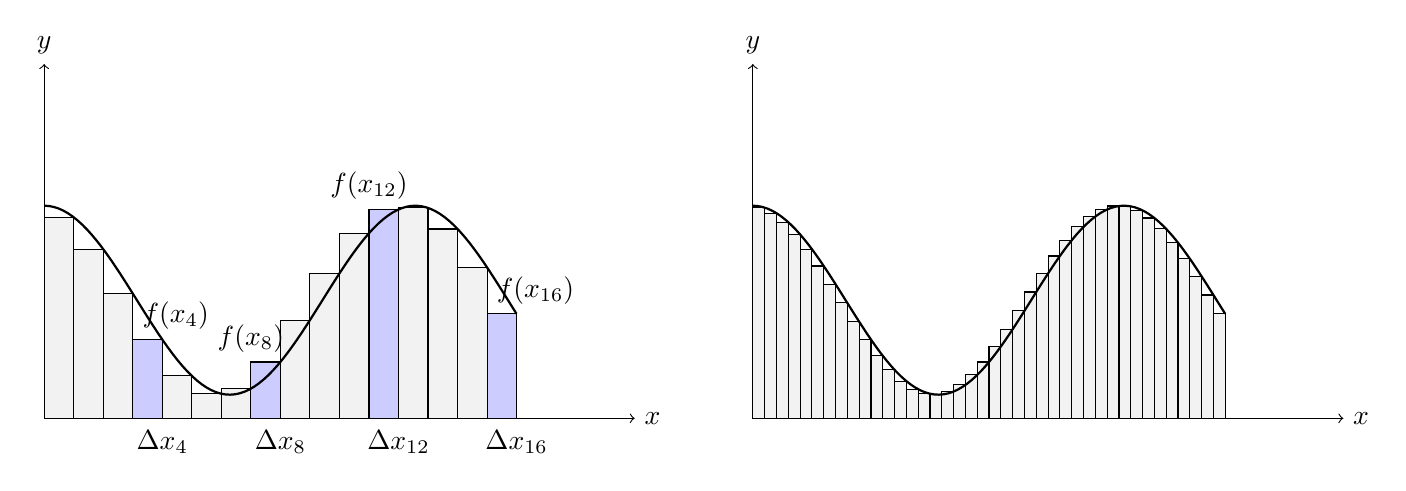
\begin{tikzpicture}[scale=1.5]
% Define the function
\def\f(#1){0.8*cos(deg(2*#1)) + 1}

% Draw the x-axis
\draw[->] (0,0) -- (5,0) node[right] {$x$};
% Draw the y-axis
\draw[->] (0,0) -- (0,3) node[above] {$y$};


% Draw the rectangles for the Riemann sum
\draw[fill=gray!10] (0, 0) rectangle (.25, {\f(.25)});
\draw[fill=gray!10] (.25, 0) rectangle (.5, {\f(.5)});
\draw[fill=gray!10] (.5, 0) rectangle (.75, {\f(.75)});
\draw[fill=blue!20] (0.75, 0) rectangle (1, {\f(1)});
\draw[fill=gray!10] (1, 0) rectangle (1.25, {\f(1.25)});
\draw[fill=gray!10] (1.25, 0) rectangle (1.5, {\f(1.5)});
\draw[fill=gray!10] (1.5, 0) rectangle (1.75, {\f(1.75)});
\draw[fill=blue!20] (1.75, 0) rectangle (2, {\f(2)});
\draw[fill=gray!10] (2, 0) rectangle (2.25, {\f(2.25)});
\draw[fill=gray!10] (2.25, 0) rectangle (2.5, {\f(2.5)});
\draw[fill=gray!10] (2.5, 0) rectangle (2.75, {\f(2.75)});
\draw[fill=blue!20] (2.75, 0) rectangle (3, {\f(3)});
\draw[fill=gray!10] (3, 0) rectangle (3.25, {\f(3.25)});
\draw[fill=gray!10] (3.25, 0) rectangle (3.5, {\f(3.5)});
\draw[fill=gray!10] (3.5, 0) rectangle (3.75, {\f(3.75)});
\draw[fill=blue!20] (3.75, 0) rectangle (4, {\f(4)});

% Draw the curve
\draw[thick, domain=0:4, samples=100] plot (\x, {\f(\x)});

% Draw the labels for f(xi)
\draw (0.75, {\f(1)}) node[above right] {$f(x_{4})$};
\draw (1.75, {\f(2)}) node[above] {$f(x_{8})$};
\draw (2.75, {\f(3)}) node[above] {$f(x_{12})$};
\draw (3.75, {\f(4)}) node[above right] {$f(x_{16})$};

% Draw the arrows for delta x

\draw (1, -0.2) node {$\Delta x_{4}$};
\draw (2, -0.2) node {$\Delta x_{8}$};
\draw (3, -0.2) node {$\Delta x_{12}$};
\draw (4, -0.2) node {$\Delta x_{16}$};

	\begin{scope}[xshift=6cm]
	% Define the function
	\def\f(#1){0.8*cos(deg(2*#1)) + 1}
	
	% Draw the x-axis
	\draw[->] (0,0) -- (5,0) node[right] {$x$};
	% Draw the y-axis
	\draw[->] (0,0) -- (0,3) node[above] {$y$};
	
	
	  % Draw the rectangles for the Riemann sum
	\foreach \xi in {0.1, 0.2, ..., 4} {
		\draw[fill=gray!10] (\xi-0.1, 0) rectangle (\xi, {\f(\xi)});
	}
	
	
	% Draw the curve
	\draw[thick, domain=0:4, samples=100] plot (\x, {\f(\x)});
	
	\end{scope}
\end{tikzpicture}
  \caption{A visualization of the Riemann Sums. The partition width is denoted by $\Delta x_i$ and the height of the partitions is $f(x_i)$.}
  \label{fig:Riemann Sum visualization}
\end{figure}

\begin{defn}[Riemann Sum\label{defn:Riemann Sum]{1}
Let $f$ be defined on the closed interval $[a,b]$, and let $\Delta$ be a partition of $[a,b]$ given by $a=x_0 < x_1 < \cdots < x_{n-1} < x_n = b$, where $\Delta x_i$ is the width of the $i$th sub-interval. If $c_i \in [x_{i-1},x_i]$, then the sum $\sum_{i=1}^{n}f(c_i)\Delta x_i$ is called a Riemann sum of $f$ for the partition $\Delta$.
\end{defn}

The largest width among the subintervals within a partition $\Delta$ is known as the partition's norm, represented by $||\Delta||$. If all subintervals have equal width, the partition is called regular, and its norm is denoted by $||\Delta|| = \Delta x = \frac{b-a}{n}$. The integral can be defined in the limit as this partition's norm approaches zero $||\Delta|| \to 0$. Therefore, there exists some $L\in\mathbf{R}$ such that for each $\epsilon > 0$, there exists a $\delta > 0$ so that for all partitions with $||\Delta|| < \delta$, we have

\begin{align}
\lim_{||\Delta|| \to 0}\sum_{i=1}^{n}f(c_i)\Delta x_i = L \implies \bigg|L-\sum_{i=1}^{n}f(c_i)\Delta x_i\bigg| < \epsilon
\end{align}

This then give the definition of the definite integral.

\begin{defn}[The Definite Integral\label{defn:The Definite Integral}]{1}
IF $f$ is defined on the closed interval $I=[a,b]$ and the limit of the Riemann sums over partitions $\Delta$ exists, then $f$ is said to be integrable on $I$ and the limit is denoted by the definite integral of $f$ from $a$ to $b$. 
\begin{align}
\lim_{||\Delta|| \to 0}\sum_{i=1}^{n}f(c_i)\Delta x_i = \int_a^b f(x)dx
\end{align}
\end{defn}

%\begin{theo}[The Fundamental Theorem Of Calculus]{1}
%Suppose that $f(x)$ is continuous on the interval [a,b]. If $F(x)$ is any antiderivative of $f(x)$, then $\int_a^b f(x) dx = F(b)-F(a)$. Given $F(x) = \int_a^b f(x) dx$, then $\frac{d}{dx}F(x) = f(x)$.
%\end{theo}
